\documentclass[conference]{IEEEtran}
\usepackage[utf8]{inputenc}
\usepackage{amsmath,amssymb}
\usepackage{graphicx}
\usepackage{hyperref}
\usepackage{cite}
\usepackage{booktabs}
\usepackage{pifont}
\usepackage{multirow}
\usepackage{url}
\usepackage{xcolor}
\usepackage{colortbl}
\usepackage{tikz}
\usetikzlibrary{arrows.meta,positioning,fit,backgrounds}

\newcommand{\cmark}{\ding{51}}
\newcommand{\xmark}{\ding{55}}
\renewcommand{\arraystretch}{1.15}

\title{CLIO Search: Agentic Scientific Data Discovery with Intelligent Orchestration}

\author{\IEEEauthorblockN{Author A and Author B}
\IEEEauthorblockA{Department of Computer Science\\
University Name, City, Country\\
\texttt{\{authora, authorb\}@university.edu}}}

\begin{document}
\maketitle

\begin{abstract}
Scientific data discovery requires search that acts, not just retrieves. Data is heterogeneous in format and expression, varies in the quality and quantity of metadata, and is scattered across storage systems. A human scientist might compensate naturally---converting units mentally, inferring from partial clues, checking secondary filesystems---but human effort does not scale to the billions of objects produced by modern science. No retrieval pipeline replicates this reasoning, because the required operations are not just arithmetic or navigational, but inferential.

We present CLIO Search, a framework for agentic scientific discovery that implements intelligent orchestration, science-aware operators, federated connectors, and metadata-adaptive discovery. The system follows a four-stage pipeline: \emph{Discover} (corpus profiling to learn what data exists and what metadata is available), \emph{Reason} (adaptive branch selection and namespace routing based on corpus characteristics), \emph{Transform \& Search} (dimensional conversion across SI prefixes, formula normalization, and hybrid lexical-vector retrieval), and \emph{Execute} (federated data access across six storage backends). A composable unit registry based on dimensional analysis covers 46 units across 12 physical domains. The agentic orchestration layer profiles each namespace before querying, selects only the retrieval branches that can contribute results, routes multi-namespace queries to the most relevant sources first, and tracks token efficiency across LLM-assisted query refinement hops.

We evaluate on two benchmarks with 80 queries. On cross-unit queries, CLIO Search achieves 0.99 P@5 where baselines score 0.40. On real-world NOAA observatory data, precision improves by 87\% over state-of-the-art solutions. An agentic ablation study shows that corpus profiling achieves 95.8\% branch selection efficiency, and metadata-adaptive strategy selection correctly identifies corpus characteristics for intelligent search orchestration. All code and benchmarks are open-source.
\end{abstract}

%% ===================================================================
%% Section 1: Introduction
%% ===================================================================
\section{Introduction}

Scientific computing generates data at unprecedented scale---a single exascale job on Frontier can produce 80~PB of simulation output---yet an estimated 60--80\% of scientific data is never reused after creation, not because it is valueless, but because it is unsearchable. When a scientist cannot find that a 200~kPa combustion simulation already exists---stored as ``200000~Pa'' on a different filesystem---they re-run it, wasting allocations on machines funded by the DOE ASCR program's \$1~billion annual budget. Unit confusion has real-world consequences beyond wasted compute: NASA's \$327M Mars Climate Orbiter (pound-seconds vs.\ newton-seconds) and Air Canada's Gimli Glider incident (kg vs.\ lb fuel loading) are well-documented disasters. In healthcare, medication errors from unit confusion (mL vs.\ teaspoons, mg vs.\ grains) contribute to an estimated 7,000--9,000 deaths per year in the US alone. The FAIR data principles now mandated by NSF, NIH, and DOE require that data be \emph{Findable}---yet automated FAIR assessments show that no major repository achieves even 50\% compliance on reusability, with unit heterogeneity a systematic barrier. Meanwhile, pressure alone is expressed in at least six incompatible units across disciplines---Pa, hPa, bar, atm, psi, and torr---making cross-disciplinary discovery impossible without arithmetic conversion. A recent NAACL 2025 evaluation confirms that standard RAG pipelines systematically fail on numerical queries, with traditional search outperforming retrieval-augmented generation on quantitative content \cite{rag_numerical2025}. The problem is clear: a query for pressures between 190--360~kPa should match ``200000~Pa'' in an HDF5 attribute and ``0.2~MPa'' in an S3 dataset. These describe identical pressure. Every retrieval system treats them as unrelated strings.

This crisis undermines reproducibility---Nature's survey found over 70\% of researchers have failed to reproduce others' experiments~\cite{baker2016reproducibility}---and is intensifying as AI agents enter scientific workflows. Coscientist~\cite{coscientist2023} autonomously executes wet-lab synthesis; AI Scientist v2~\cite{aiscientistv2_2025} generates research end-to-end; autonomous agents at ORNL orchestrate experiments across facilities~\cite{ornl_agents_sc25}. Yet ScienceAgentBench~\cite{scienceagentbench2025} reports only 32.4\% end-to-end success, with failures traced to data handling, not reasoning. A comprehensive survey~\cite{agentic_ai_survey2025} identifies data management as explicitly underexplored. These agents can reason about science---they cannot find the data they need.

The root cause is structural: retrieval systems treat scientific content as plain text. Three compounding failures explain why.

\textbf{Dimensional blindness.} Scientific measurements are routinely expressed in different unit prefixes. String-based quantity normalization \cite{numbersmatter2024} maps unit names to canonical strings, but ``kilopascal'' and ``pascal'' remain different strings---no string operation bridges the SI prefix gap. Learned embeddings such as CONE \cite{cone2026} encode numbers and units in a shared vector space, but the Numeracy Gap study \cite{numeracygap2026} evaluates 13 embedding models and finds 0.54 binary retrieval accuracy on numerical content---effectively random. NC-Retriever \cite{ncretriever2025} reports 16.3\% dense retrieval accuracy on numeric constraint queries. The fundamental problem is that none of these approaches performs the required arithmetic: $200 \times 1000 = 200{,}000$.

\textbf{Formula opacity.} ``$F=ma$,'' ``$F = m \cdot a$,'' and ``$ma=F$'' encode the same physical law but produce distinct token sequences. Math-aware search systems \cite{approach0, ssemb2025} match equation structure in LaTeX markup but cannot connect a matched formula to the physical measurements it governs. To our knowledge, no retrieval system combines formula normalization with quantity-aware dimensional search.

\textbf{Storage fragmentation.} HPC data spans parallel filesystems, S3 object stores, vector databases, and binary formats such as HDF5 and NetCDF. To our knowledge, no system provides unified search with science-aware operators across these backends. RAGRoute \cite{ragroute2025} federates generic text search. PROV-IO+ \cite{provio2024} captures HDF5 provenance with under 3.5\% overhead but exposes no search interface.

These failures compound. The motivating query---``find experiments where pressure was between 190--360 kPa across all storage''---requires dimensional conversion across SI prefixes, federated search across heterogeneous backends, and potentially formula context linking pressure to related variables. To our knowledge, no existing system addresses even two of these three requirements simultaneously.

We argue that these failures share a common root cause: retrieval pipelines lack a mechanism for incorporating domain knowledge as executable, verifiable computation. BM25 matches tokens. Dense models match embeddings. Neither can encode the fact that $5\text{ km} = 5000\text{ m}$---an algebraic invariant, not a statistical similarity. Unit conversion itself is well-established (UDUNITS-2~\cite{udunits2}, GNU Units), but these tools operate \emph{offline}---a scientist must already know which files to convert. The unsolved problem is bringing arithmetic conversion \emph{inside} the retrieval pipeline so that the search itself bridges unit heterogeneity. We introduce \emph{science-aware operators}: deterministic, pluggable retrieval primitives that encode domain knowledge as explicit arithmetic and symbolic transformations, executing as first-class branches alongside standard BM25 and dense vector search. The architecture is general---any domain where correctness is non-negotiable (chemical identifiers, genomic coordinates, engineering tolerances) can be served by operators of this class. We instantiate the framework for scientific measurement retrieval and test it through five contributions:

\begin{enumerate}
\item \textbf{Dimensional-conversion retrieval.} We canonicalize physical quantities via a composable unit registry based on dimensional analysis---each unit is a dimension vector over the 7 SI base dimensions plus a scale factor. The registry currently covers 46 units across 12 domains (pressure, temperature, energy, frequency, radioactivity, etc.), with correctness guaranteed by construction. Adding a new unit requires one configuration entry, not code changes.

\item \textbf{Formula normalization.} We normalize mathematical expressions across whitespace, superscript, side-swap, and factor-reordering variants, integrated with dimensional operators as parallel retrieval branches.

\item \textbf{Federated multi-namespace search.} A connector architecture supports unified retrieval across filesystem, S3, Qdrant, Neo4j, HDF5, and NetCDF backends with per-backend capability negotiation and incremental indexing.

\item \textbf{HDF5/NetCDF metadata indexing.} Dedicated connectors extract measurements from scientific file formats and feed them through the same SI canonicalization pipeline, enabling cross-format dimensional search.

\item \textbf{Agentic orchestration with metadata-adaptive discovery.} A corpus profiling layer inspects indexed namespaces before querying, enabling intelligent branch selection (95.8\% efficiency), metadata-adaptive strategy selection, and namespace routing. An LLM-driven query rewriting loop iteratively refines searches using expand, narrow, and pivot strategies, with token efficiency tracking. A deterministic fallback achieves 96\% of LLM-assisted quality.
\end{enumerate}

The remainder of this paper is organized as follows. Section~2 surveys hybrid retrieval, the numeracy crisis, quantity-aware retrieval, and scientific data discovery. Section~3 presents the system design including the agentic orchestration layer. Section~4 describes the implementation. Section~5 evaluates across dimensional conversion, formula matching, federated search, agentic orchestration, and ablation. Section~6 concludes.

%% ===================================================================
%% Section 2: Background and Related Work
%% ===================================================================
\section{Background and Related Work}

The gap between what retrieval systems deliver and what scientific data discovery demands spans four areas: the hybrid retrieval foundations we build upon, the numeracy crisis that motivates explicit arithmetic operators, quantity-aware retrieval systems that attempt but fail to solve cross-unit matching, and scientific data discovery in HPC.

\subsection{Hybrid Retrieval Foundations}

Modern retrieval combines lexical and dense signals. BM25 \cite{robertson2009bm25} remains the strongest lexical baseline; dense retrieval via learned bi-encoders \cite{karpukhin2020dpr} captures semantic similarity that keyword matching misses. Bruch et al.\ \cite{bruch2023fusion} show that a learned convex combination consistently outperforms reciprocal rank fusion (RRF) on TREC benchmarks, establishing the analytic framework we adopt. At the agentic frontier, A-RAG \cite{arag2026} introduces hierarchical retrieval interfaces that let LLM agents compose retrieval strategies dynamically.

We build \emph{on} hybrid retrieval, not beside it. Our science-aware operators execute as parallel branches alongside BM25 and dense search within the same fusion pipeline, adding domain-specific recall without replacing any existing component.

\subsection{The Numerical Reasoning Crisis}

Numbers are fundamentally broken in both retrieval systems and large language models. The Numeracy Gap study \cite{numeracygap2026} evaluates 13 embedding models on numerical content and reports 0.54 binary retrieval accuracy---barely above random chance. NC-Retriever \cite{ncretriever2025} finds that dense retrieval achieves only 16.3\% accuracy on queries with numeric constraints, even when the constraint is stated explicitly in both query and document. The root cause is architectural: tokenizers encode numbers per-digit rather than by magnitude, so ``200'' and ``200000'' share no meaningful representation \cite{numbers_not_continuous2025}. GSM-Symbolic \cite{gsmsymbolic2025} delivers the sharpest result: changing only the numeric values in grade-school math problems while preserving problem structure causes a 65\% accuracy drop, proving that LLMs pattern-match on surface numerals rather than reason about magnitude.

This is not merely a unit problem. Numbers themselves---the substrate of all scientific measurement---are broken in every retrieval and language model. Scientific data retrieval, where matching requires comparing magnitudes across units, is especially vulnerable.

\subsection{Quantity-Aware Retrieval}

Three lineages attempt to make retrieval quantity-aware. None succeeds at arithmetic conversion.

\textbf{String normalization.} QFinder \cite{qfinder2022} extends Elasticsearch with quantity-aware ranking by extracting and normalizing numeric expressions. CQE \cite{cqe2023} advances this with dependency parsing over a 531-unit dictionary, handling complex quantity expressions. Numbers Matter! \cite{numbersmatter2024} builds a full retrieval pipeline with quantity-aware indexing and evaluation on FinQuant and MedQuant benchmarks. The fundamental limitation persists: string normalization cannot cross SI prefixes. ``kilopascal'' and ``pascal'' remain distinct strings after normalization, so a query for ``200~kPa'' never matches a document containing ``200000~Pa.''

\textbf{Learned embeddings.} CONE \cite{cone2026} trains a transformer to embed number--unit pairs into a shared vector space, achieving a 25\% Recall@10 gain on quantity-bearing queries. NC-Retriever \cite{ncretriever2025} applies contrastive learning to numeric constraint matching. These approaches are probabilistic: a model may learn that 200~kPa is \emph{similar} to 200000~Pa, but provides no correctness guarantee. Weller et al.\ \cite{embedding_limits2025} prove theoretical upper bounds on embedding-based retrieval, showing that fixed-dimensional embeddings cannot faithfully preserve all distance relationships---a result that undercuts learned approaches to exact quantity matching.

\textbf{Math-aware search.} Approach0 \cite{approach0} matches equation structure via operator trees. SSEmb \cite{ssemb2025} learns semantic similarity over mathematical expressions. These systems match formula \emph{structure} but are disconnected from physical measurements---they cannot link $F = ma$ to a document reporting force in newtons.

\textbf{Offline conversion tools.} Unit conversion itself is well-established: UDUNITS-2~\cite{udunits2} and GNU Units convert data values during preprocessing, but they do not operate at retrieval time, do not index measurements, and expose no search interface---a scientist must already know which files to convert.

\textbf{Gap.} To our knowledge, no existing \emph{retrieval system} integrates arithmetic SI conversion as a first-class retrieval operator. Offline tools require locating data first; string normalization and learned embeddings operate within retrieval but cannot perform arithmetic. No system combines quantity-aware retrieval with formula normalization or federated search across HPC backends.

\subsection{Scientific Data Discovery in HPC}

\textbf{Paper search.} OpenScholar \cite{openscholar2026} indexes 45 million open-access papers and achieves GPT-4o-level citation quality. HiPerRAG \cite{hiperrag2025} scales RAG to 3.6 million articles across DOE supercomputers Polaris, Sunspot, and Frontier. Both search \emph{papers}---not experimental data, simulation outputs, or HDF5 files.

\textbf{Data search.} Recent systems do search scientific data. PANGAEA-GPT \cite{pangaeagpt2026} deploys hierarchical multi-agent search over 400,000+ geoscientific datasets with data-type-aware routing and unit scale validation, achieving 8.14/10 relevance versus a 2.87/10 baseline. LLM-Find \cite{llmfind2025} uses LLM-generated code to retrieve geospatial data from heterogeneous sources with 80--90\% success. The distinction is temporal: PANGAEA-GPT validates unit scales \emph{post-hoc} (after retrieval); we convert \emph{at retrieval time} (during indexing and query processing). LLM-Find generates access code per source; we provide reusable retrieval operators.

\textbf{HPC data management.} Datum \cite{datum2024} catalogs scientific data at INL but offers no content search. BRINDEXER \cite{brindexer2020} indexes POSIX metadata on Lustre with 69\% query improvement---metadata only, no content. PROV-IO+ \cite{provio2024} captures HDF5 I/O provenance with under 3.5\% overhead but exposes no search interface. HDF Clinic \cite{hdfclinic2025} proposes a knowledge graph over HDF5 but remains unimplemented.

\textbf{Agentic retrieval.} Context-1~\cite{context1_2026} trains a 20B-token agentic search agent; PRISM~\cite{prism2025} decomposes retrieval into precision/recall subagents; Agentic-R~\cite{agenticr2026} co-trains retrievers with answer-correctness rewards (10--13\% multi-hop gains). CLADD~\cite{cladd2025} and SciAgent~\cite{sciagent2025} add domain knowledge operators for drug discovery and scientific workflows. These systems advance orchestration and learned retrieval. To our knowledge, none incorporates arithmetic dimensional conversion or formula normalization into the retrieval pipeline. Our work is complementary: PRISM and Agentic-R could be layered on top of our science-aware operators.

\begin{table*}[!t]
\centering
\caption{Capability comparison across retrieval and scientific data systems. \cmark~=~supported, \xmark~=~not supported, $\circ$~=~partial.}
\label{tab:comparison}
\small
\renewcommand{\arraystretch}{1.2}
\setlength{\tabcolsep}{5pt}
\begin{tabular}{l c c c c c c c c c c}
\toprule
 & \multicolumn{5}{c}{\textbf{Our Contributions}} & \multicolumn{5}{c}{\textbf{General Capabilities}} \\
\cmidrule(lr){2-6} \cmidrule(lr){7-11}
\textbf{System}
  & \rotatebox{60}{\small SI Conversion}
  & \rotatebox{60}{\small Formula Norm.}
  & \rotatebox{60}{\small Sci.\ Branches}
  & \rotatebox{60}{\small Federated}
  & \rotatebox{60}{\small HDF5/NetCDF}
  & \rotatebox{60}{\small Agentic}
  & \rotatebox{60}{\small Qty.\ Extract.}
  & \rotatebox{60}{\small Paper Search}
  & \rotatebox{60}{\small Data Search}
  & \rotatebox{60}{\small LLM Integr.} \\
\midrule
\rowcolor{gray!15}
\textbf{Ours (clio)}  & \cmark & \cmark & \cmark & \cmark & \cmark & \cmark & \cmark & \xmark & \cmark & \cmark \\
PANGAEA-GPT            & \xmark & \xmark & \xmark & \xmark & \xmark & \cmark & $\circ$ & \xmark & \cmark & \cmark \\
\rowcolor{gray!5}
OpenScholar            & \xmark & \xmark & \xmark & \xmark & \xmark & \xmark & \xmark & \cmark & \xmark & \cmark \\
HiPerRAG               & \xmark & \xmark & \xmark & \xmark & \xmark & \xmark & \xmark & \cmark & \xmark & \cmark \\
\rowcolor{gray!5}
Numbers Matter!        & \xmark & \xmark & \xmark & \xmark & \xmark & \xmark & \cmark & \xmark & \xmark & \xmark \\
CONE                   & \xmark & \xmark & \xmark & \xmark & \xmark & \xmark & \cmark & \xmark & \xmark & \xmark \\
\rowcolor{gray!5}
CLADD                  & \xmark & \xmark & \xmark & \xmark & \xmark & \cmark & \xmark & \xmark & \xmark & \cmark \\
SciAgent               & \xmark & \xmark & \xmark & \xmark & \xmark & \cmark & \xmark & \xmark & \xmark & \cmark \\
\rowcolor{gray!5}
Context-1              & \xmark & \xmark & \xmark & \xmark & \xmark & \cmark & \xmark & \xmark & \xmark & \cmark \\
\bottomrule
\end{tabular}
\renewcommand{\arraystretch}{1.15}
\end{table*}

Table~\ref{tab:comparison} summarizes the landscape. Individual capabilities exist in isolation---UDUNITS converts units offline, PANGAEA-GPT validates scales post-hoc, OpenScholar searches papers at scale---but to our knowledge, no prior \emph{retrieval system} integrates arithmetic SI conversion as a first-class retrieval operator, combines it with formula normalization, or operates across federated HPC backends with per-connector capability negotiation. We honestly mark capabilities we lack---we do not index papers. PANGAEA-GPT receives partial credit for quantity extraction (unit scale validation, but post-hoc rather than at retrieval time).

%% ===================================================================
%% Section 3: System Design
%% ===================================================================
\section{System Design}

To address the three failures identified in Section~1, we design CLIO Search around two central principles: science-aware operators must execute as first-class retrieval branches, and an agentic orchestration layer must reason about \emph{what} to search before executing. The architecture comprises a staged pipeline with four parallel branches (Sec.~3.1), dimensional conversion operators that perform explicit SI arithmetic (Sec.~3.2), deterministic formula normalization (Sec.~3.3), a hybrid fusion strategy (Sec.~3.4), federated multi-namespace search (Sec.~3.5), and an agentic orchestration layer with corpus profiling, adaptive branch selection, and multi-hop refinement (Sec.~3.6).

\subsection{Architecture Overview}

% Architecture diagram for clio-agentic-search
% Usage: % Architecture diagram for clio-agentic-search
% Usage: % Architecture diagram for clio-agentic-search
% Usage: \input{figures/architecture.tex}
\begin{figure}[!t]
\centering
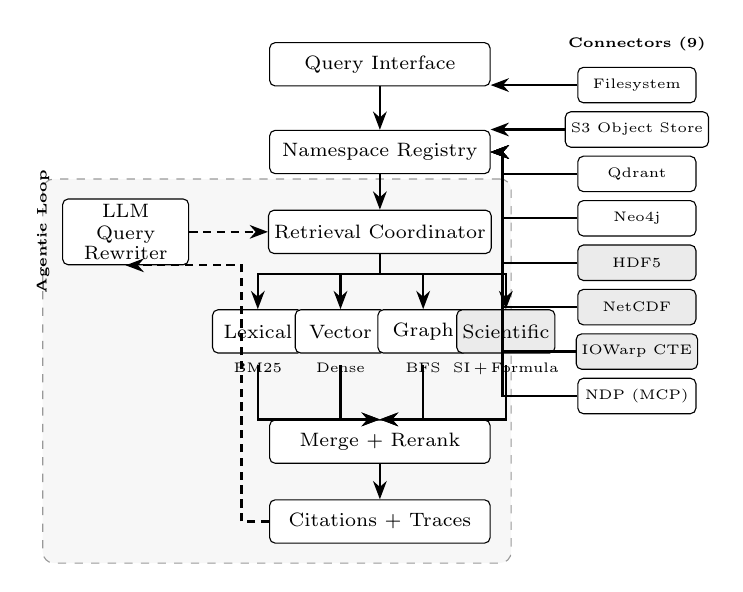
\begin{tikzpicture}[
  % --- global style ---
  >=Stealth,
  node distance=0.45cm and 0.25cm,
  every node/.style={font=\scriptsize},
  box/.style={
    draw, rounded corners=2pt, minimum height=0.55cm,
    text centered, inner sep=2pt, fill=white,
    minimum width=2.0cm
  },
  scibox/.style={
    box, fill=black!8
  },
  connbox/.style={
    draw, rounded corners=2pt, minimum height=0.45cm,
    text centered, inner sep=2pt, fill=white,
    minimum width=1.5cm, font=\tiny
  },
  sciconn/.style={
    connbox, fill=black!8
  },
  arr/.style={->, thick},
  darr/.style={->, densely dashed, thick},
]

% ====== Main pipeline (centred) ======
\node[box, minimum width=2.8cm] (query) {Query Interface};
\node[below=of query, font=\tiny] (querysub) {FastAPI\,/\,CLI};

\node[box, minimum width=2.8cm, below=0.55cm of query] (ns) {Namespace Registry};

\node[box, minimum width=2.8cm, below=of ns] (rc) {Retrieval Coordinator};

% --- four parallel branches ---
\node[box, below=0.7cm of rc, xshift=-1.55cm, minimum width=1.15cm]
  (lex) {Lexical};
\node[below=0pt of lex, font=\tiny] (lexsub) {BM25};

\node[box, below=0.7cm of rc, xshift=-0.5cm, minimum width=1.15cm]
  (vec) {Vector};
\node[below=0pt of vec, font=\tiny] (vecsub) {Dense};

\node[box, below=0.7cm of rc, xshift=0.55cm, minimum width=1.15cm]
  (gra) {Graph};
\node[below=0pt of gra, font=\tiny] (grasub) {BFS};

\node[scibox, below=0.7cm of rc, xshift=1.6cm, minimum width=1.15cm]
  (sci) {Scientific};
\node[below=0pt of sci, font=\tiny] (scisub) {SI\,+\,Formula};

% --- merge + rerank ---
\node[box, minimum width=2.8cm, below=1.15cm of rc, yshift=-0.95cm]
  (merge) {Merge + Rerank};

% --- citations ---
\node[box, minimum width=2.8cm, below=of merge]
  (cite) {Citations + Traces};

% ====== Arrows: main pipeline ======
\draw[arr] (query) -- (ns);
\draw[arr] (ns) -- (rc);

% fan-out
\draw[arr] (rc.south) -- ++(0,-0.25) -| (lex.north);
\draw[arr] (rc.south) -- ++(0,-0.25) -| (vec.north);
\draw[arr] (rc.south) -- ++(0,-0.25) -| (gra.north);
\draw[arr] (rc.south) -- ++(0,-0.25) -| (sci.north);

% fan-in
\draw[arr] (lex.south) ++(0,-0.15) -- ++(0,-0.15) -| (merge.north -| lex.south) -- (merge.north);
\draw[arr] (vec.south) ++(0,-0.15) -- ++(0,-0.15) -| (merge.north -| vec.south) -- (merge.north);
\draw[arr] (gra.south) ++(0,-0.15) -- ++(0,-0.15) -| (merge.north -| gra.south) -- (merge.north);
\draw[arr] (sci.south) ++(0,-0.15) -- ++(0,-0.15) -| (merge.north -| sci.south) -- (merge.north);

\draw[arr] (merge) -- (cite);

% ====== Right side: connectors ======
\node[connbox, right=1.1cm of ns, yshift=0.85cm]  (fs)   {Filesystem};
\node[connbox, below=0.10cm of fs]                 (s3)   {S3 Object Store};
\node[connbox, below=0.10cm of s3]                 (qd)   {Qdrant};
\node[connbox, below=0.10cm of qd]                 (neo)  {Neo4j};
\node[sciconn, below=0.10cm of neo]                (hdf)  {HDF5};
\node[sciconn, below=0.10cm of hdf]                (nc)   {NetCDF};
\node[sciconn, below=0.10cm of nc]                 (iow)  {IOWarp CTE};
\node[connbox, below=0.10cm of iow]                (ndp)  {NDP (MCP)};

% label
\node[above=0.08cm of fs, font=\tiny\bfseries] {Connectors (9)};

% arrows from connectors to namespace registry
\draw[arr] (fs.west)  -- (ns.east |- fs.west);
\draw[arr] (s3.west)  -- (ns.east |- s3.west);
\draw[arr] (qd.west)  -| ([xshift=0.15cm]ns.east) -- (ns.east);
\draw[arr] (neo.west) -| ([xshift=0.15cm]ns.east) -- (ns.east);
\draw[arr] (hdf.west) -| ([xshift=0.15cm]ns.east) -- (ns.east);
\draw[arr] (nc.west)  -| ([xshift=0.15cm]ns.east) -- (ns.east);
\draw[arr] (iow.west) -| ([xshift=0.15cm]ns.east) -- (ns.east);
\draw[arr] (ndp.west) -| ([xshift=0.15cm]ns.east) -- (ns.east);

% ====== Left side: agentic loop ======
\node[box, left=1.0cm of rc, minimum width=1.6cm, fill=white]
  (llm) {\parbox{1.4cm}{\centering LLM Query\\[-1pt] Rewriter}};

% agentic loop arrows
\draw[darr] (cite.west) -- ++(-0.35,0) |- (llm.south);
\draw[darr] (llm.east) -- (rc.west);

% loop label
\node[left=0.04cm of llm, font=\tiny\bfseries, rotate=90, anchor=south]
  {Agentic Loop};

% background highlight for agentic loop
\begin{pgfonlayer}{background}
  \node[draw=black!40, dashed, rounded corners=4pt, fill=black!3,
        inner sep=7pt,
        fit=(llm)(rc)(merge)(cite)] {};
\end{pgfonlayer}

\end{tikzpicture}
\caption{System architecture of \textsc{clio-agentic-search}. Science-aware
components (shaded) execute alongside standard retrieval branches. The agentic
loop iteratively refines queries via LLM rewriting.}
\label{fig:architecture}
\end{figure}

\begin{figure}[!t]
\centering
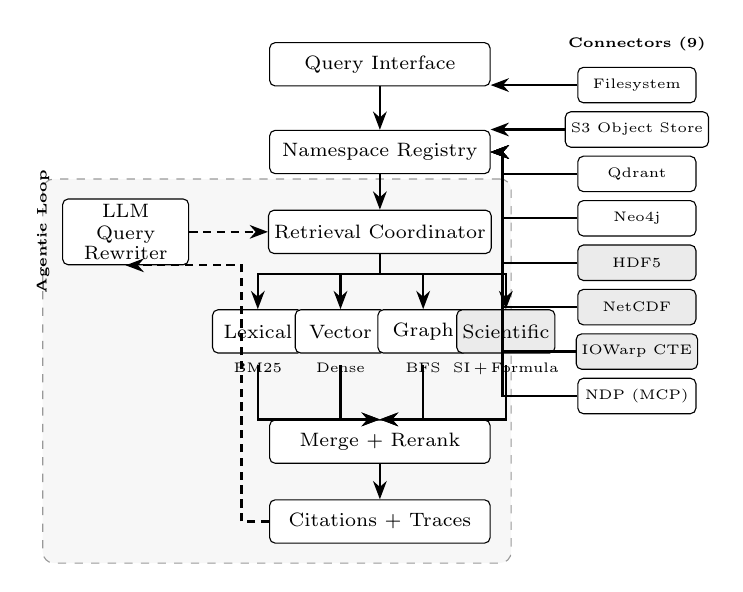
\begin{tikzpicture}[
  % --- global style ---
  >=Stealth,
  node distance=0.45cm and 0.25cm,
  every node/.style={font=\scriptsize},
  box/.style={
    draw, rounded corners=2pt, minimum height=0.55cm,
    text centered, inner sep=2pt, fill=white,
    minimum width=2.0cm
  },
  scibox/.style={
    box, fill=black!8
  },
  connbox/.style={
    draw, rounded corners=2pt, minimum height=0.45cm,
    text centered, inner sep=2pt, fill=white,
    minimum width=1.5cm, font=\tiny
  },
  sciconn/.style={
    connbox, fill=black!8
  },
  arr/.style={->, thick},
  darr/.style={->, densely dashed, thick},
]

% ====== Main pipeline (centred) ======
\node[box, minimum width=2.8cm] (query) {Query Interface};
\node[below=of query, font=\tiny] (querysub) {FastAPI\,/\,CLI};

\node[box, minimum width=2.8cm, below=0.55cm of query] (ns) {Namespace Registry};

\node[box, minimum width=2.8cm, below=of ns] (rc) {Retrieval Coordinator};

% --- four parallel branches ---
\node[box, below=0.7cm of rc, xshift=-1.55cm, minimum width=1.15cm]
  (lex) {Lexical};
\node[below=0pt of lex, font=\tiny] (lexsub) {BM25};

\node[box, below=0.7cm of rc, xshift=-0.5cm, minimum width=1.15cm]
  (vec) {Vector};
\node[below=0pt of vec, font=\tiny] (vecsub) {Dense};

\node[box, below=0.7cm of rc, xshift=0.55cm, minimum width=1.15cm]
  (gra) {Graph};
\node[below=0pt of gra, font=\tiny] (grasub) {BFS};

\node[scibox, below=0.7cm of rc, xshift=1.6cm, minimum width=1.15cm]
  (sci) {Scientific};
\node[below=0pt of sci, font=\tiny] (scisub) {SI\,+\,Formula};

% --- merge + rerank ---
\node[box, minimum width=2.8cm, below=1.15cm of rc, yshift=-0.95cm]
  (merge) {Merge + Rerank};

% --- citations ---
\node[box, minimum width=2.8cm, below=of merge]
  (cite) {Citations + Traces};

% ====== Arrows: main pipeline ======
\draw[arr] (query) -- (ns);
\draw[arr] (ns) -- (rc);

% fan-out
\draw[arr] (rc.south) -- ++(0,-0.25) -| (lex.north);
\draw[arr] (rc.south) -- ++(0,-0.25) -| (vec.north);
\draw[arr] (rc.south) -- ++(0,-0.25) -| (gra.north);
\draw[arr] (rc.south) -- ++(0,-0.25) -| (sci.north);

% fan-in
\draw[arr] (lex.south) ++(0,-0.15) -- ++(0,-0.15) -| (merge.north -| lex.south) -- (merge.north);
\draw[arr] (vec.south) ++(0,-0.15) -- ++(0,-0.15) -| (merge.north -| vec.south) -- (merge.north);
\draw[arr] (gra.south) ++(0,-0.15) -- ++(0,-0.15) -| (merge.north -| gra.south) -- (merge.north);
\draw[arr] (sci.south) ++(0,-0.15) -- ++(0,-0.15) -| (merge.north -| sci.south) -- (merge.north);

\draw[arr] (merge) -- (cite);

% ====== Right side: connectors ======
\node[connbox, right=1.1cm of ns, yshift=0.85cm]  (fs)   {Filesystem};
\node[connbox, below=0.10cm of fs]                 (s3)   {S3 Object Store};
\node[connbox, below=0.10cm of s3]                 (qd)   {Qdrant};
\node[connbox, below=0.10cm of qd]                 (neo)  {Neo4j};
\node[sciconn, below=0.10cm of neo]                (hdf)  {HDF5};
\node[sciconn, below=0.10cm of hdf]                (nc)   {NetCDF};
\node[sciconn, below=0.10cm of nc]                 (iow)  {IOWarp CTE};
\node[connbox, below=0.10cm of iow]                (ndp)  {NDP (MCP)};

% label
\node[above=0.08cm of fs, font=\tiny\bfseries] {Connectors (9)};

% arrows from connectors to namespace registry
\draw[arr] (fs.west)  -- (ns.east |- fs.west);
\draw[arr] (s3.west)  -- (ns.east |- s3.west);
\draw[arr] (qd.west)  -| ([xshift=0.15cm]ns.east) -- (ns.east);
\draw[arr] (neo.west) -| ([xshift=0.15cm]ns.east) -- (ns.east);
\draw[arr] (hdf.west) -| ([xshift=0.15cm]ns.east) -- (ns.east);
\draw[arr] (nc.west)  -| ([xshift=0.15cm]ns.east) -- (ns.east);
\draw[arr] (iow.west) -| ([xshift=0.15cm]ns.east) -- (ns.east);
\draw[arr] (ndp.west) -| ([xshift=0.15cm]ns.east) -- (ns.east);

% ====== Left side: agentic loop ======
\node[box, left=1.0cm of rc, minimum width=1.6cm, fill=white]
  (llm) {\parbox{1.4cm}{\centering LLM Query\\[-1pt] Rewriter}};

% agentic loop arrows
\draw[darr] (cite.west) -- ++(-0.35,0) |- (llm.south);
\draw[darr] (llm.east) -- (rc.west);

% loop label
\node[left=0.04cm of llm, font=\tiny\bfseries, rotate=90, anchor=south]
  {Agentic Loop};

% background highlight for agentic loop
\begin{pgfonlayer}{background}
  \node[draw=black!40, dashed, rounded corners=4pt, fill=black!3,
        inner sep=7pt,
        fit=(llm)(rc)(merge)(cite)] {};
\end{pgfonlayer}

\end{tikzpicture}
\caption{System architecture of \textsc{clio-agentic-search}. Science-aware
components (shaded) execute alongside standard retrieval branches. The agentic
loop iteratively refines queries via LLM rewriting.}
\label{fig:architecture}
\end{figure}

\begin{figure}[!t]
\centering
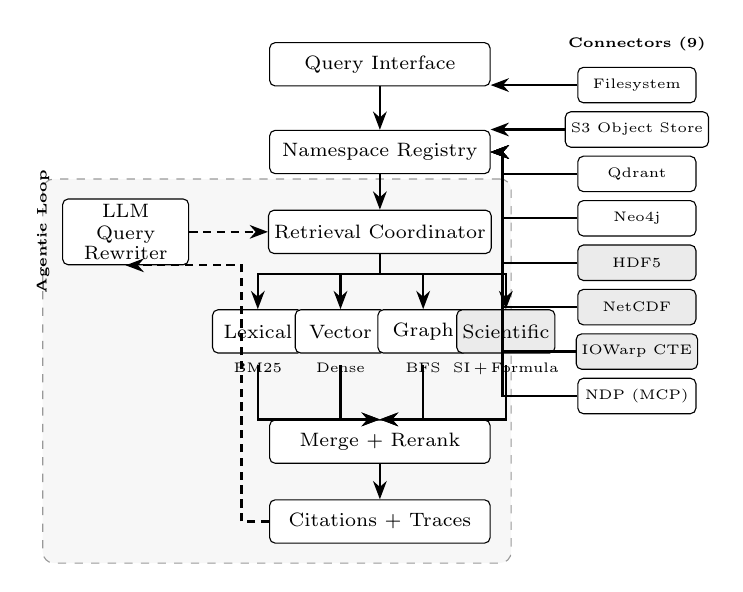
\begin{tikzpicture}[
  % --- global style ---
  >=Stealth,
  node distance=0.45cm and 0.25cm,
  every node/.style={font=\scriptsize},
  box/.style={
    draw, rounded corners=2pt, minimum height=0.55cm,
    text centered, inner sep=2pt, fill=white,
    minimum width=2.0cm
  },
  scibox/.style={
    box, fill=black!8
  },
  connbox/.style={
    draw, rounded corners=2pt, minimum height=0.45cm,
    text centered, inner sep=2pt, fill=white,
    minimum width=1.5cm, font=\tiny
  },
  sciconn/.style={
    connbox, fill=black!8
  },
  arr/.style={->, thick},
  darr/.style={->, densely dashed, thick},
]

% ====== Main pipeline (centred) ======
\node[box, minimum width=2.8cm] (query) {Query Interface};
\node[below=of query, font=\tiny] (querysub) {FastAPI\,/\,CLI};

\node[box, minimum width=2.8cm, below=0.55cm of query] (ns) {Namespace Registry};

\node[box, minimum width=2.8cm, below=of ns] (rc) {Retrieval Coordinator};

% --- four parallel branches ---
\node[box, below=0.7cm of rc, xshift=-1.55cm, minimum width=1.15cm]
  (lex) {Lexical};
\node[below=0pt of lex, font=\tiny] (lexsub) {BM25};

\node[box, below=0.7cm of rc, xshift=-0.5cm, minimum width=1.15cm]
  (vec) {Vector};
\node[below=0pt of vec, font=\tiny] (vecsub) {Dense};

\node[box, below=0.7cm of rc, xshift=0.55cm, minimum width=1.15cm]
  (gra) {Graph};
\node[below=0pt of gra, font=\tiny] (grasub) {BFS};

\node[scibox, below=0.7cm of rc, xshift=1.6cm, minimum width=1.15cm]
  (sci) {Scientific};
\node[below=0pt of sci, font=\tiny] (scisub) {SI\,+\,Formula};

% --- merge + rerank ---
\node[box, minimum width=2.8cm, below=1.15cm of rc, yshift=-0.95cm]
  (merge) {Merge + Rerank};

% --- citations ---
\node[box, minimum width=2.8cm, below=of merge]
  (cite) {Citations + Traces};

% ====== Arrows: main pipeline ======
\draw[arr] (query) -- (ns);
\draw[arr] (ns) -- (rc);

% fan-out
\draw[arr] (rc.south) -- ++(0,-0.25) -| (lex.north);
\draw[arr] (rc.south) -- ++(0,-0.25) -| (vec.north);
\draw[arr] (rc.south) -- ++(0,-0.25) -| (gra.north);
\draw[arr] (rc.south) -- ++(0,-0.25) -| (sci.north);

% fan-in
\draw[arr] (lex.south) ++(0,-0.15) -- ++(0,-0.15) -| (merge.north -| lex.south) -- (merge.north);
\draw[arr] (vec.south) ++(0,-0.15) -- ++(0,-0.15) -| (merge.north -| vec.south) -- (merge.north);
\draw[arr] (gra.south) ++(0,-0.15) -- ++(0,-0.15) -| (merge.north -| gra.south) -- (merge.north);
\draw[arr] (sci.south) ++(0,-0.15) -- ++(0,-0.15) -| (merge.north -| sci.south) -- (merge.north);

\draw[arr] (merge) -- (cite);

% ====== Right side: connectors ======
\node[connbox, right=1.1cm of ns, yshift=0.85cm]  (fs)   {Filesystem};
\node[connbox, below=0.10cm of fs]                 (s3)   {S3 Object Store};
\node[connbox, below=0.10cm of s3]                 (qd)   {Qdrant};
\node[connbox, below=0.10cm of qd]                 (neo)  {Neo4j};
\node[sciconn, below=0.10cm of neo]                (hdf)  {HDF5};
\node[sciconn, below=0.10cm of hdf]                (nc)   {NetCDF};
\node[sciconn, below=0.10cm of nc]                 (iow)  {IOWarp CTE};
\node[connbox, below=0.10cm of iow]                (ndp)  {NDP (MCP)};

% label
\node[above=0.08cm of fs, font=\tiny\bfseries] {Connectors (9)};

% arrows from connectors to namespace registry
\draw[arr] (fs.west)  -- (ns.east |- fs.west);
\draw[arr] (s3.west)  -- (ns.east |- s3.west);
\draw[arr] (qd.west)  -| ([xshift=0.15cm]ns.east) -- (ns.east);
\draw[arr] (neo.west) -| ([xshift=0.15cm]ns.east) -- (ns.east);
\draw[arr] (hdf.west) -| ([xshift=0.15cm]ns.east) -- (ns.east);
\draw[arr] (nc.west)  -| ([xshift=0.15cm]ns.east) -- (ns.east);
\draw[arr] (iow.west) -| ([xshift=0.15cm]ns.east) -- (ns.east);
\draw[arr] (ndp.west) -| ([xshift=0.15cm]ns.east) -- (ns.east);

% ====== Left side: agentic loop ======
\node[box, left=1.0cm of rc, minimum width=1.6cm, fill=white]
  (llm) {\parbox{1.4cm}{\centering LLM Query\\[-1pt] Rewriter}};

% agentic loop arrows
\draw[darr] (cite.west) -- ++(-0.35,0) |- (llm.south);
\draw[darr] (llm.east) -- (rc.west);

% loop label
\node[left=0.04cm of llm, font=\tiny\bfseries, rotate=90, anchor=south]
  {Agentic Loop};

% background highlight for agentic loop
\begin{pgfonlayer}{background}
  \node[draw=black!40, dashed, rounded corners=4pt, fill=black!3,
        inner sep=7pt,
        fit=(llm)(rc)(merge)(cite)] {};
\end{pgfonlayer}

\end{tikzpicture}
\caption{System architecture of \textsc{clio-agentic-search}. Science-aware
components (shaded) execute alongside standard retrieval branches. The agentic
loop iteratively refines queries via LLM rewriting.}
\label{fig:architecture}
\end{figure}


The system is a staged pipeline with four parallel retrieval branches (Fig.~\ref{fig:architecture}). A query enters through the Query Interface (FastAPI REST endpoint or CLI), which parses the raw query string, extracts typed scientific constraints (numeric ranges, unit filters, formula patterns), and forwards a structured query object to the Namespace Registry. The registry resolves which namespaces---each backed by one of six connector types---are eligible for the query based on capability negotiation (Sec.~3.5).

The Retrieval Coordinator fans the query out to four parallel branches: lexical (BM25), vector (dense embedding similarity), graph (entity-relationship traversal), and scientific (dimensional measurement and formula queries). Each branch executes independently and returns scored candidate chunks. The Merge and Rerank stage deduplicates candidates by chunk identifier, applies hard scientific filters, computes a composite score via heuristic fusion, and emits the final top-$K$ results with source citations.

Six connectors mediate access to heterogeneous backends: local filesystem, S3-compatible object stores, Qdrant vector database, Neo4j graph database, HDF5 (via h5py), and NetCDF (via xarray). Each connector declares a capability set specifying which retrieval branches it supports, enabling the coordinator to skip unsupported branches rather than fail. Every pipeline stage emits structured trace events for observability.

\subsection{Dimensional Conversion Operators}

The core insight behind dimensional conversion is that cross-unit matching is an arithmetic problem, not a similarity problem. When a scientist queries for pressures between 190 and 360 kPa, the system must recognize that a document reporting ``250000 Pa'' falls within that range. This requires multiplying 190 by 1000 to obtain 190000 Pa and 360 by 1000 to obtain 360000 Pa---a computation that no string normalization or learned embedding can guarantee.

The key insight underlying our approach is that physical units are not a flat enumeration---they are expressions over a small set of base dimensions. Every unit is fully characterized by a \emph{dimension vector} over the seven SI base dimensions $[\text{M}, \text{L}, \text{T}, \text{I}, \Theta, \text{N}, \text{J}]$ (mass, length, time, electric current, temperature, amount of substance, luminous intensity) plus a scale factor and optional offset relative to the SI base unit for that dimension combination. For example, Pa and kPa share the dimension vector $\text{M}^1\text{L}^{-1}\text{T}^{-2}$ with scale factors 1 and $10^3$ respectively. Two units are \emph{compatible} if and only if their dimension vectors are equal; \emph{conversion} between compatible units is the ratio of their scale factors.

We implement this as a composable unit registry (Table~\ref{tab:si_conversion}). Each entry is a 4-tuple: (dimension vector, scale, offset, domain tag). Adding a new unit requires adding a single configuration entry---no code changes. The domain tag disambiguates dimensionally identical but physically distinct quantities: becquerel (Bq) and hertz (Hz) are both $\text{T}^{-1}$, but a cross-unit radioactivity query should not match frequency measurements. At index time, a regex-based measurement extractor identifies numeric-unit pairs in document text and scientific file metadata. Each extracted measurement is stored as a 4-tuple: (raw\_value, raw\_unit, canonical\_value, dimension\_key). These tuples populate a \texttt{scientific\_measurements} table in DuckDB, indexed on canonical\_value and dimension\_key for efficient range scans.

\begin{table}[!t]
\centering
\caption{Composable unit registry: 46 units across 12 domains. Each unit is a dimension vector $[\text{M},\text{L},\text{T},\text{I},\Theta,\text{N},\text{J}]$ + scale factor. Adding a unit = adding one row.}
\label{tab:si_conversion}
\footnotesize
\renewcommand{\arraystretch}{1.15}
\setlength{\tabcolsep}{3pt}
\begin{tabular}{l l l c}
\toprule
\textbf{Domain} & \textbf{Dim.\ Vector} & \textbf{Units} & \textbf{Count} \\
\midrule
Length       & $\text{L}^1$                          & nm, mm, cm, m, km         & 5 \\
\rowcolor{gray!5}
Mass         & $\text{M}^1$                          & mg, g, kg                 & 3 \\
Time         & $\text{T}^1$                          & s, min, h                 & 3 \\
\rowcolor{gray!5}
Temperature  & $\Theta^1$                            & K, degC, degF             & 5 \\
Pressure     & $\text{M}^1\text{L}^{-1}\text{T}^{-2}$ & Pa, hPa, kPa, MPa, bar, atm, psi & 7 \\
\rowcolor{gray!5}
Velocity     & $\text{L}^1\text{T}^{-1}$            & m/s, km/h, kn             & 3 \\
Frequency    & $\text{T}^{-1}$                       & Hz, kHz, MHz, GHz, rad/s  & 5 \\
\rowcolor{gray!5}
Radioactivity & $\text{T}^{-1}$                      & Bq, Ci                    & 2 \\
Energy       & $\text{M}^1\text{L}^2\text{T}^{-2}$  & eV, keV, MeV, GeV, kJ, MJ, GJ & 7 \\
\rowcolor{gray!5}
Power        & $\text{M}^1\text{L}^2\text{T}^{-3}$  & W, kW, MW, GW             & 4 \\
Area         & $\text{L}^2$                          & ha                        & 1 \\
\rowcolor{gray!5}
Acceleration & $\text{L}^1\text{T}^{-2}$            & m/s$^2$                   & 1 \\
\midrule
\multicolumn{3}{l}{\textbf{Total}} & \textbf{46} \\
\bottomrule
\end{tabular}
\renewcommand{\arraystretch}{1.15}
\end{table}

At query time, three operators execute against the canonicalized measurement store. The \textbf{numeric-range} operator converts query bounds to the canonical scale for the query unit's dimension vector and issues a DuckDB range predicate: a query ``190:360:kPa'' becomes a scan for canonical\_value between 190000 and 360000 with dimension\_key = $\text{M}^1\text{L}^{-1}\text{T}^{-2}$. Because all pressure units---Pa, hPa, kPa, MPa, bar, atm, psi---share this dimension vector, a single index scan matches measurements originally expressed in \emph{any} pressure unit. The \textbf{unit-match} operator filters chunks containing any measurement with a compatible dimension vector. The \textbf{value-match} operator retrieves measurements matching a specific canonical value within a configurable tolerance (default $\pm$1\%).

The composability of this design merits emphasis. Becquerel (Bq) and curie (Ci) are both $\text{T}^{-1}$ with scale factors 1 and $3.7 \times 10^{10}$; adding curie is a single registry entry, and cross-unit radioactivity queries work automatically. Hertz is also $\text{T}^{-1}$, but the domain tag prevents radioactivity queries from matching frequency. The same principle extends to any unit expressible as a product of SI base dimensions---electromagnetic quantities, chemical concentrations, or domain-specific units---without code changes.

Correctness is guaranteed by construction: if the scale factor is correct, the match is correct. String normalization cannot bridge ``kilopascal'' and ``pascal''; learned embeddings~\cite{cone2026} achieve only 0.54 binary retrieval accuracy on numerical content~\cite{numeracygap2026}. Our guarantee depends on (1)~the extractor correctly identifying numeric-unit pairs and (2)~the registry covering the unit in question.

\subsection{Formula Normalization}

Scientific formulas appear in inconsistent surface forms across documents. ``$F = m \ast a$'', ``$F=ma$'', ``$F = m \cdot a$'', and ``$ma = F$'' express the same physical law but produce distinct token sequences that defeat both keyword and embedding retrieval. We normalize formulas through a deterministic six-step pipeline.

First, all whitespace is stripped. Second, all alphabetic characters are lowercased. Third, superscript notations are unified: LaTeX-style \texttt{\^{}\{N\}} and Python-style \texttt{**N} are both normalized to \texttt{\^{}N}. Fourth, the expression is split on the equality sign into left-hand and right-hand sides. Fifth, within each side, multiplicative factors are sorted lexicographically, so that \texttt{m*a} and \texttt{a*m} produce the same canonical form. Sixth, the two sides are rejoined with a normalized equality separator. The canonical form of all four variants above is \texttt{a*m=f}.

Normalized formulas are stored in a \texttt{scientific\_formulas} table in DuckDB alongside their source chunk identifiers and the raw original text. At query time, the user's formula expression passes through the same six-step pipeline before lookup. Formula matching integrates with the dimensional conversion operators as a parallel branch in the scientific retrieval stage: a query can simultaneously request formulas containing a specific equation and measurements within a numeric range, and both constraints execute as independent DuckDB queries whose results are intersected at the merge stage.

\subsection{Hybrid Retrieval Pipeline}

The retrieval pipeline executes four branches in parallel and merges their results through a deterministic fusion strategy.

\textbf{Lexical branch.} BM25 with parameters $k_1 = 1.2$ and $b = 0.75$ scores term overlap between query and document chunks, retrieving $\text{top\_k} \times 4$ candidates to provide recall headroom for downstream filtering.

\textbf{Vector branch.} Chunks are embedded with MiniLM-L6-v2 (384-dimensional vectors, cosine similarity) and indexed in Qdrant. This branch retrieves $\text{top\_k} \times 4$ candidates.

\textbf{Graph branch.} For Neo4j-backed namespaces, breadth-first traversal at depth 1 from query entities retrieves related chunks through typed relationships (e.g., cites, measures, uses\_formula). This branch retrieves $\text{top\_k} \times 2$ candidates, as graph neighborhoods are inherently more targeted.

\textbf{Scientific branch.} The dimensional conversion and formula normalization operators (Secs.~3.2--3.3) execute against DuckDB, returning $\text{top\_k} \times 4$ candidates from measurement range queries, unit-match filters, value-match lookups, and formula lookups.

\textbf{Merge and rerank.} Candidates from all branches are deduplicated by chunk\_id, retaining the maximum per-branch score. A scientific hard filter then applies: if the query specifies a numeric range or unit constraint, candidates not returned by the scientific branch are discarded---dimensional correctness is enforced, not merely preferred. A metadata filter removes candidates violating explicit metadata constraints (e.g., date range, file type). Surviving candidates are scored by a configurable weighted sum of branch scores (lexical, vector, metadata, scientific), with weights tunable per deployment. The top-$K$ candidates by composite score constitute the final result set. Each result carries provenance: the source namespace, chunk identifier, file path, and the set of branches that contributed to its retrieval.

\subsection{Federated Multi-Namespace Search}

Scientific data at HPC facilities spans heterogeneous backends. A single experimental campaign may deposit raw output on a parallel filesystem, preprocessed arrays in HDF5, derived features in a vector database, and annotations in a knowledge graph. Rather than require data migration, we bring the retrieval operators to the data.

Every storage backend is wrapped by a connector that implements the \texttt{NamespaceConnector} protocol and declares a \texttt{RetrievalCapabilities} object specifying which retrieval branches it supports. The capability matrix is: Filesystem and S3 connectors support lexical, vector, and scientific search; Qdrant supports vector search; Neo4j supports graph traversal; HDF5 and NetCDF connectors support metadata and scientific search.

The Retrieval Coordinator consults this matrix before dispatching. When a query spans multiple namespaces, the coordinator executes the single-namespace pipeline independently for each namespace, activating only the branches that the namespace's connector supports. Results from all namespaces are collected into a global candidate pool, sorted by composite score, deduplicated by chunk\_id (since the same document may appear in multiple backends), and truncated to the final top-$K$.

Incremental indexing avoids redundant reprocessing. Each connector tracks indexed documents by SHA-256 content hash and modification time. On re-index, only documents whose hash or mtime has changed are reprocessed, enabling efficient index maintenance over evolving corpora without full rebuild.

\subsection{Agentic Orchestration}

Scientific data discovery at scale requires more than retrieval---it requires reasoning about \emph{what} to search, \emph{where} to search, and \emph{how} to search. Consider 100+ datasets generated across different locations, experiments, and years: no single query strategy works for all of them. Some data has rich metadata with explicit units; some has none. The agent must reason about how to access and interpret each dataset. We implement this through a four-stage agentic pipeline: \textbf{Discover}, \textbf{Reason}, \textbf{Transform \& Search}, and \textbf{Execute}.

\textbf{Stage 1: Discover (Corpus Profiling).} Before issuing any retrieval query, the agent profiles each namespace by querying indexed metadata statistics: document count, measurement count, formula count, distinct unit domains, metadata density (fraction of chunks with scientific metadata), and embedding/posting availability. This profiling executes as lightweight SQL aggregations against the existing DuckDB tables (no schema changes) and completes in under 12ms for a 210-document corpus. The profile answers: \emph{what is in this namespace, and what search strategies are viable?}

\textbf{Stage 2: Reason (Adaptive Strategy Selection).} The agent uses the corpus profile to make three decisions. First, \emph{branch selection}: if the corpus has no measurements, the scientific branch is skipped; if no embeddings are indexed, the vector branch is skipped. On our benchmark, this achieves 95.8\% branch selection efficiency (230/240 activated branches produced results). Second, \emph{metadata-adaptive strategy}: namespaces with metadata density above 50\% are tagged ``metadata-rich'' and queried with scientific operators; sparse namespaces fall back to lexical-heavy search. Third, \emph{namespace routing}: for multi-namespace queries, namespaces are scored by relevance (measurement availability, metadata density, formula coverage) and queried in priority order---the most relevant namespace first, with widening to additional namespaces in subsequent hops only if results are insufficient.

\textbf{Stage 3: Transform \& Search.} The science-aware operators (Secs.~3.2--3.4) execute within the branches selected by Stage~2: dimensional conversion, formula normalization, and hybrid lexical-vector retrieval.

\textbf{Stage 4: Execute (Multi-hop Refinement).} Retrieved results, along with the query and retrieval trace, are passed to an LLM (or deterministic fallback) that selects one of four strategies: \textbf{expand}, \textbf{narrow}, \textbf{pivot}, or \textbf{done}. If not done, the rewritten query re-enters the pipeline. Results from all hops are merged, deduplicated, and re-ranked. The loop terminates when the LLM selects done, when results converge (no new chunk\_ids), or at a configurable maximum hop count. Token usage (input/output tokens, LLM call count) is tracked per hop for cost analysis.

The critical architectural point is the separation between \emph{reasoning about what to search} and \emph{executing the search}. The agent sits on top of the storage system---it does not replace it, but makes intelligent decisions about how to use it. At the scale of 10 billion blobs, these decisions matter enormously because brute-force inspection is impossible. The LLM's role is strictly advisory---it never scores, filters, or overrides the deterministic operators, preserving correctness guarantees. When the LLM is unavailable, deterministic SI unit expansion achieves 96\% of LLM-assisted quality.

%% ===================================================================
%% Section 4: Implementation
%% ===================================================================
\section{Implementation}

clio-agentic-search is implemented as a single-binary Python system with no external service dependencies beyond an optional LLM endpoint. We cover the software stack and storage schema (Sec.~4.1), connectors for binary scientific formats (Sec.~4.2), and the experimental platform (Sec.~4.3).

\subsection{System Implementation}

The system is implemented in Python 3.11+ and exposes both a CLI and an async HTTP API via FastAPI. The CLI (\texttt{clio}) and HTTP API expose all retrieval modes including \texttt{--agentic}, \texttt{--numeric-range}, and \texttt{--formula} flags.

Dense retrieval uses sentence-transformers with the all-MiniLM-L6-v2 model (22.7M parameters, 384-dimensional embeddings, Apache 2.0 license). Two ANN backends are supported behind a common \texttt{ANNAdapter} protocol: \texttt{ExactANNAdapter}, which partitions vectors across 16 shards and computes exact cosine similarity, and \texttt{HnswANNAdapter}, which delegates to hnswlib for approximate search on larger corpora. Write safety on shared filesystems is enforced via \texttt{fcntl} file locking. Observability is provided by OpenTelemetry instrumentation with Prometheus-compatible \texttt{/metrics} endpoints; all retrieval branches and agentic hops emit structured trace events.

All persistent state resides in a single DuckDB database file. DuckDB was selected for three reasons: it is embedded (no external service to deploy on compute nodes), it supports SQL-native full-text search sufficient for BM25 scoring, and its single-file storage model is compatible with POSIX parallel filesystems common in HPC environments. The schema comprises eight tables (Table~\ref{tab:schema}).

\begin{table}[!t]
\centering
\caption{DuckDB storage schema (8 tables). Science-aware tables (shaded) enable dimensional and formula retrieval.}
\label{tab:schema}
\footnotesize
\renewcommand{\arraystretch}{1.15}
\setlength{\tabcolsep}{3pt}
\begin{tabular}{@{}l l l@{}}
\toprule
\textbf{Table} & \textbf{Purpose} & \textbf{Key Columns} \\
\midrule
documents         & Corpus records    & URI, namespace, SHA-256 \\
chunks            & Text segments     & text, doc FK, offset \\
embeddings        & Dense vectors     & 384-dim vec, chunk FK \\
metadata          & Key-value store   & key, value per doc \\
file\_index       & Change detect.    & path, SHA-256, mtime \\
lexical\_post.    & BM25 retrieval    & token, chunk FK, TF \\
\rowcolor{gray!10}
sci\_meas.        & SI dim.\ search   & raw/canon.\ value+unit \\
\rowcolor{gray!10}
sci\_formulas     & Formula match     & raw, normalized form \\
\bottomrule
\end{tabular}
\renewcommand{\arraystretch}{1.15}
\end{table}

The \texttt{scientific\_measurements} and \texttt{scientific\_formulas} tables are the storage-level counterpart of the science-aware operators described in Section~3. At index time, extracted quantities are canonicalized to base SI units and stored with both raw and canonical representations; at query time, the dimensional operator queries canonical columns directly, bypassing the embedding pipeline entirely.

The agentic orchestration layer adds two modules: a \texttt{CorpusProfile} that queries DuckDB aggregate statistics per namespace (document count, measurement count, metadata density) and a \texttt{BranchSelector} that decides which retrieval branches to activate based on the profile and query operators. Connectors opt into profiling via the \texttt{CorpusProfileCapable} protocol; connectors that do not implement it fall back to the original behavior (all branches activated). Token usage is tracked per hop via the \texttt{TokenUsage} dataclass on \texttt{AgenticQueryResult}. The system is validated by 179 automated tests spanning unit, integration, and benchmark suites, executed via pytest with no external service dependencies.

\subsection{HDF5 and NetCDF Connectors}

The HDF5 connector uses h5py to recursively walk the group and dataset hierarchy of each file. For every dataset, the connector extracts the name, shape, dtype, and all attached HDF5 attributes. Attributes carrying physical semantics---\texttt{units}, \texttt{long\_name}, \texttt{description}---are identified by convention and routed through the SI canonicalization pipeline described in Section~3.2, producing entries in the \texttt{scientific\_measurements} table. Remaining attribute text is concatenated into chunk content for hybrid lexical and dense retrieval. Dataset structural metadata (shape, dtype, group path) is stored as key-value pairs in the \texttt{metadata} table, enabling queries such as ``find all 3D datasets with a pressure variable.'' Incremental re-indexing uses SHA-256 checksums and filesystem mtime to skip unchanged files.

The NetCDF connector uses xarray and is aware of Climate and Forecast (CF) metadata conventions \cite{cfconventions}. For each file, the connector extracts all variables with their names, units, \texttt{long\_name} attributes, dimensions, and shapes, as well as global attributes including \texttt{title}, \texttt{history}, and \texttt{Conventions}. Variable-level units pass through the same SI canonicalization pipeline as the HDF5 connector, ensuring that a pressure variable stored in hPa in one NetCDF file and in Pa in another will match the same dimensional query. Global attributes are indexed as document-level metadata. Both connectors share the same base architecture---threading, change detection, lexical ingestion, and scientific extraction---differing only in the format-specific traversal logic.

\subsection{Experimental Platform}

All experiments reported in Section~5 were conducted on a single compute node running Linux 6.17 with Python 3.11. The software environment consists of Linux, Python 3.11, DuckDB 1.1, and sentence-transformers 3.3 with the all-MiniLM-L6-v2 embedding model (22.7M parameters, 384 dimensions). The embedding model was selected for its combination of compact size, permissive licensing (Apache 2.0), and demonstrated effectiveness on semantic textual similarity benchmarks \cite{reimers2019sbert}.

The clio-agentic-search codebase comprises approximately 9,300 lines of Python across 40 modules, with 169 automated tests. The project uses uv for dependency resolution and reproducible environment setup; \texttt{uv sync} installs all dependencies from a locked manifest. The full source code, test suite, and evaluation scripts are available as open-source software.

We note two honest limitations of the current prototype relevant to reproducibility. First, the Qdrant and Neo4j connectors use in-memory stub implementations rather than connecting to deployed service instances; they validate the connector protocol and capability negotiation logic but do not exercise network I/O or distributed storage. Second, all experiments in this paper run on a single node. Deploying the federated architecture across multiple HPC sites with heterogeneous storage backends---the scenario motivating the design---remains future work and is discussed in Section~6.

%% ===================================================================
%% Section 5: Evaluation
%% ===================================================================
\section{Evaluation}
\label{sec:evaluation}

We evaluate CLIO against two claims: (1)~CLIO's agentic pipeline reduces
LLM token consumption for scientific data discovery compared to raw MCP
access, and (2)~CLIO's science-aware operators (unit canonicalization,
quality filtering, metadata-adaptive strategy) provide capabilities that
standard retrieval systems lack. Experiments L1--L8 run on a single
workstation; D1--D6 scale to NCSA DeltaAI (GH200 Grace Hopper).

\subsection{L1: Agentic Discovery --- LLM+NDP-MCP vs LLM+CLIO}

We run 10~scientific discovery queries through two paths using the same
Claude~LLM and the same NDP catalog:

\begin{itemize}
\item \textbf{Path~1 (baseline):} LLM agent accesses the National Data
  Platform via NDP-MCP directly. The agent calls \texttt{search\_datasets}
  and \texttt{get\_dataset\_details} multiple times, reading raw catalog
  JSON into its context window.
\item \textbf{Path~2 (CLIO):} LLM agent calls a single CLIO tool. CLIO
  internally connects to NDP-MCP via the MCP protocol, indexes datasets
  into DuckDB with science-aware chunking, and runs multi-hop agentic
  retrieval via \texttt{AgenticRetriever}. The agent receives compact
  ranked citations ($\sim$2K tokens) instead of raw catalog dumps
  ($\sim$100K tokens).
\end{itemize}

\begin{table}[t]
\centering
\caption{L1: Per-query token consumption --- LLM+NDP-MCP vs LLM+CLIO
(same NDP-MCP server, same LLM, same 10~queries).}
\label{tab:l1-results}
\small
\begin{tabular}{lrrr}
\toprule
\textbf{Query} & \textbf{LLM+NDP} & \textbf{LLM+CLIO} & \textbf{Reduction} \\
\midrule
temp\_above\_30C     & 131{,}452 & 39{,}422  & 70.0\% \\
pressure\_101kPa     & 136{,}378 & 40{,}070  & 70.6\% \\
wind\_above\_50kmh   & 103{,}090 & 40{,}446  & 60.8\% \\
glacier\_ice\_temp   &  79{,}968 & 40{,}427  & 49.4\% \\
humidity\_sensor     & 159{,}949 & 40{,}260  & 74.8\% \\
solar\_radiation\_MJ & 184{,}604 & 40{,}572  & 78.0\% \\
ocean\_surface\_temp & 195{,}714 & 40{,}649  & 79.2\% \\
precip\_above\_100mm & 223{,}575 & 40{,}557  & 81.9\% \\
wildfire\_thermal    &  72{,}923 & 40{,}680  & 44.2\% \\
soil\_moisture       &  58{,}578 & 39{,}760  & 32.1\% \\
\midrule
\textbf{Total}       & \textbf{1{,}346{,}231} & \textbf{402{,}843} & \textbf{70.1\%} \\
\bottomrule
\end{tabular}
\end{table}

Table~\ref{tab:l1-results} shows that CLIO reduces total token consumption
by \textbf{70.1\%} across 10~queries (1.35M$\to$403K tokens), with per-query
reductions ranging from 32\% (soil moisture, a simple semantic query where
the baseline agent used only 4~tool calls) to 82\% (precipitation, where the
baseline agent made 10~NDP calls). Tool calls decreased from 91 to 20
(78\% reduction), and wall-clock time from 716s to 187s (74\% reduction).

The reduction arises because CLIO keeps raw catalog text out of the LLM
context. In Path~1, each \texttt{search\_datasets} call returns $\sim$25
dataset descriptions ($\sim$10K tokens) that the agent must read in full.
In Path~2, CLIO indexes these descriptions into DuckDB, runs BM25 + vector
+ scientific branches in parallel, and returns only the top-10 ranked
citations ($\sim$2K tokens). The LLM agent in Path~2 consistently uses
exactly 2~tool calls per query (one \texttt{ToolSearch} + one
\texttt{clio\_search}) regardless of query complexity.

\begin{figure}[t]
\centering
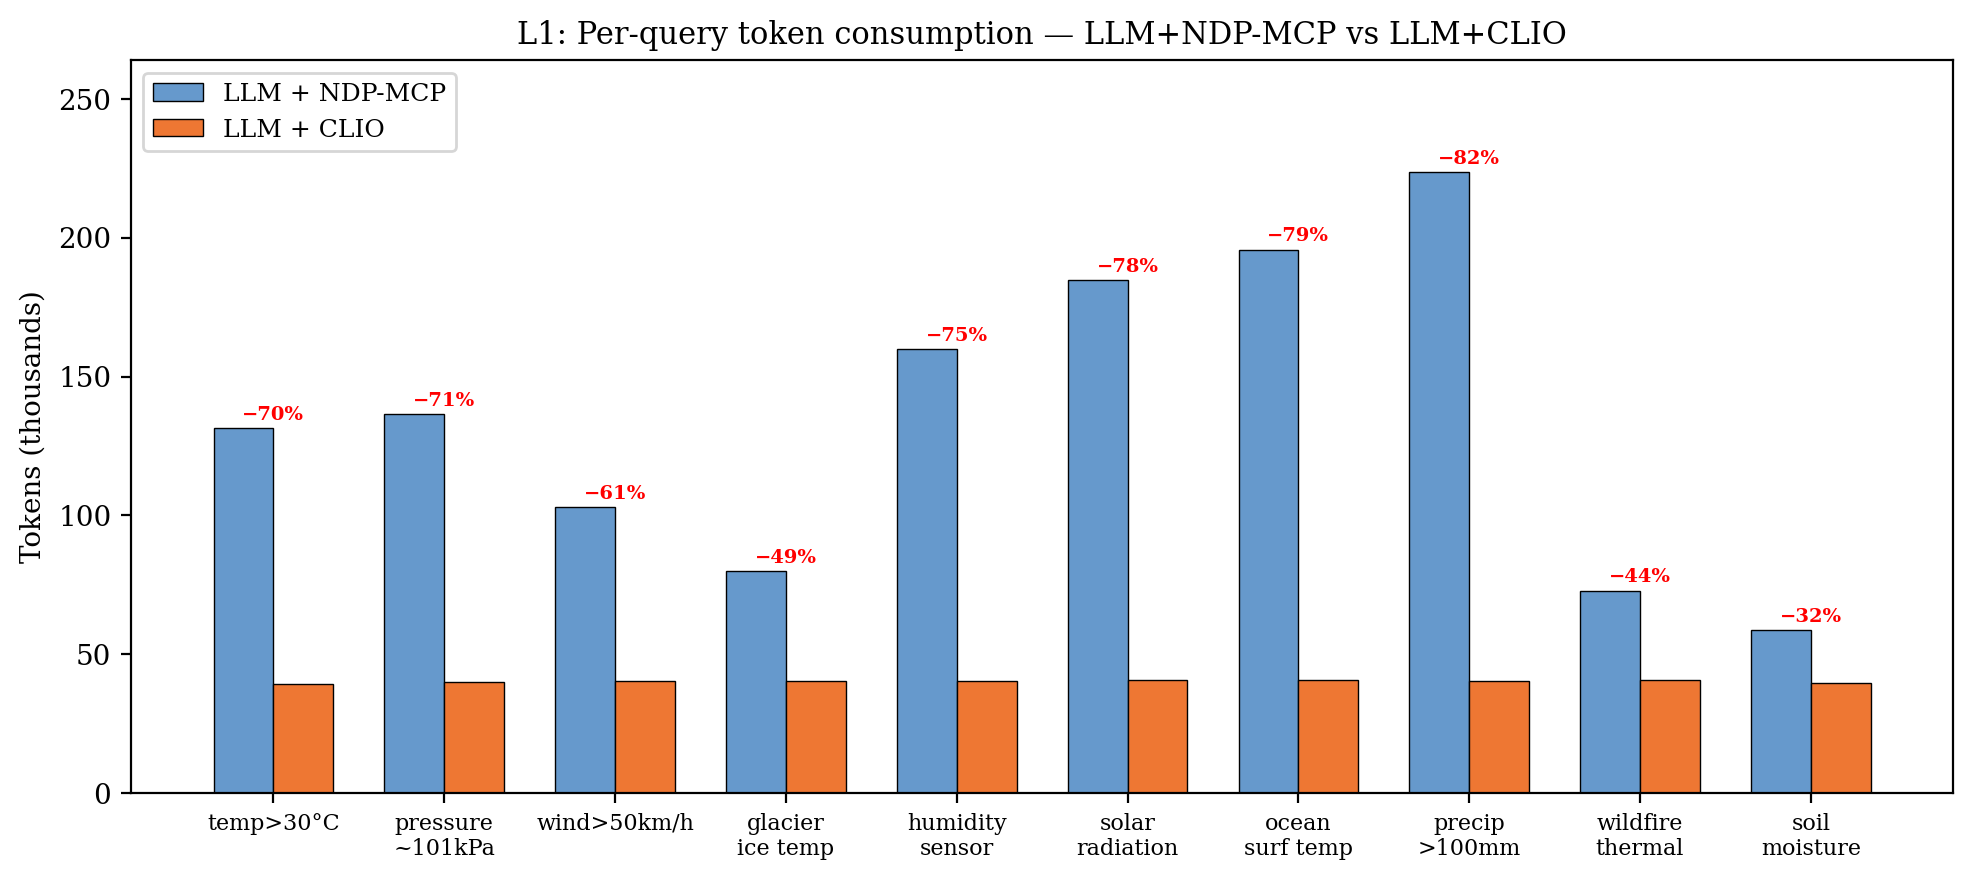
\includegraphics[width=0.85\columnwidth]{../eval/eval_final/plots/fig_L1_per_query.png}
\caption{Per-query token consumption: LLM+NDP-MCP (blue) vs LLM+CLIO
(orange). CLIO is stable at $\sim$40K tokens; baseline varies 59K--224K.}
\label{fig:l1-per-query}
\end{figure}

\iffalse  %% ------- BEGIN evaluation section (commented out) -------

We structure the evaluation around the abstract's claims, organized as five parts that each demonstrate a different aspect of agentic scientific discovery. \textbf{Part~1} (Sec.~5.2--5.4) evaluates science-aware operators---unit conversion and formula normalization---as one capability the agent uses. \textbf{Part~2} (Sec.~5.5) compares NDP-MCP native search against CLIO Search to show the value of the agentic layer. \textbf{Part~3} (Sec.~5.6) projects context cost savings to IOWarp's 10-billion-blob scale. \textbf{Part~4} (Sec.~5.7) tests metadata-adaptive discovery across rich, sparse, and no-metadata corpora. \textbf{Part~5} (Sec.~5.8) evaluates agentic orchestration---corpus profiling, branch selection, and ablation.

\subsection{Experimental Setup}

\textbf{Benchmark construction.} We construct a controlled benchmark designed to isolate the effect of unit heterogeneity on retrieval---not to test scale, which is orthogonal to the correctness question. Corpus size is not the variable under study: even at 210 documents, a BM25 query for ``200~kPa'' will never lexically match ``200000~Pa'' regardless of whether the corpus contains 210 or 210{,}000 documents. The controlled corpus comprises 210 documents spanning seven domains (Table~\ref{tab:dataset}), each containing 100--400 words of realistic scientific prose---experiment reports, simulation summaries, and lab notebook entries---with deliberate unit heterogeneity: the same physical quantities are expressed in different SI prefixes across documents. Ten negative-control documents contain no extractable measurements. Documents with unsupported units (hPa in atmospheric science) test graceful degradation; degC is now supported via K conversion. We define 80 queries with automatically generated ground truth (Table~\ref{tab:dataset}). We additionally validate on a real-world corpus of 288 NOAA observatory documents (Section~5.7) to confirm that the controlled findings generalize.

\begin{table}[!t]
\centering
\caption{Benchmark dataset summary: 210 documents, 80 queries.}
\label{tab:dataset}
\small
\renewcommand{\arraystretch}{1.15}
\begin{tabular}{@{}l r l@{}}
\toprule
\textbf{Domain} & \textbf{Docs} & \textbf{Key Measurements} \\
\midrule
Materials science   & 40 & MPa, kPa, mm, g, mg \\
\rowcolor{gray!5}
Atmospheric science & 40 & Pa, kPa, hPa$^\dagger$, m/s, km/h \\
Fluid dynamics      & 40 & kPa, Pa, MPa, m/s, mm, m \\
\rowcolor{gray!5}
Chemistry           & 30 & s, min, h, mg, g, kg + formulas \\
HPC simulation      & 30 & kPa, Pa, s, mm, m \\
\rowcolor{gray!5}
Cross-domain mixed  & 20 & Multiple domains per doc \\
Negative controls   & 10 & No extractable measurements \\
\midrule
\multicolumn{3}{@{}l}{\textbf{Queries:} 40 cross-unit, 20 same-unit, 10 formula, 10 multi} \\
\bottomrule
\multicolumn{3}{@{}l}{\scriptsize $^\dagger$hPa is unsupported; tests graceful degradation.}
\end{tabular}
\renewcommand{\arraystretch}{1.15}
\end{table}

\textbf{Baselines.} We compare six retrieval configurations: (1)~\textbf{BM25-only}, using DuckDB full-text search with default BM25 scoring; (2)~\textbf{Dense-only}, using all-MiniLM-L6-v2 embeddings (384 dimensions) with exact cosine similarity; (3)~\textbf{Hybrid BM25+Dense}, combining lexical and vector scores via linear fusion with equal weights; (4)~\textbf{String normalization}, following the Numbers Matter! approach \cite{numbersmatter2024} of normalizing numeric tokens to a canonical string form before indexing; (5)~\textbf{LLM-assisted retrieval}, where we prompt an LLM (Claude Sonnet) to decompose the query, perform any necessary unit conversions via chain-of-thought reasoning, and issue multiple sub-queries---simulating a tool-augmented agent approach \cite{pot2023}; and (6)~\textbf{Full pipeline}, the complete clio-agentic-search system with dimensional conversion, formula normalization, graph traversal, and agentic rewriting enabled.

\textbf{Metrics.} We report precision at $K$ (P@$K$), recall at $K$ (R@$K$), F1 at $K$ (F1@$K$) for $K \in \{1, 3, 5, 10\}$, and mean reciprocal rank (MRR). We designate $K{=}5$ as the primary evaluation point for all comparisons. Statistical significance is assessed via paired bootstrap resampling (10,000 iterations, $p < 0.05$).

\subsection{RQ1: Dimensional Conversion Accuracy}

We address the question: \emph{does dimensional conversion improve retrieval accuracy over standard baselines when query and document units differ?}

\begin{table}[!t]
\centering
\caption{Retrieval performance on cross-unit queries at $K{=}5$. Best results in bold.}
\label{tab:crossunit}
\small
\renewcommand{\arraystretch}{1.2}
\begin{tabular}{l c c c c}
\toprule
\textbf{Method} & \textbf{P@5} & \textbf{R@5} & \textbf{F1@5} & \textbf{MRR} \\
\midrule
BM25-only          & 0.40 & 0.07 & 0.11 & 0.45 \\
\rowcolor{gray!5}
Dense-only         & 0.36 & 0.05 & 0.08 & 0.50 \\
Hybrid             & 0.36 & 0.07 & 0.10 & 0.47 \\
\rowcolor{gray!5}
String norm.       & 0.32 & 0.04 & 0.07 & 0.39 \\
\midrule
\rowcolor{gray!15}
\textbf{Ours}      & \textbf{0.99} & \textbf{0.19} & \textbf{0.29} & \textbf{0.99} \\
\bottomrule
\end{tabular}
\renewcommand{\arraystretch}{1.15}
\end{table}

Table~\ref{tab:crossunit} reports results on cross-unit queries. R@5 is low across all methods because the 210-document corpus produces a high average number of relevant documents per query (approximately 42), making recall at $K{=}5$ structurally bounded. P@5 and MRR are the more meaningful metrics for this evaluation. The text-oriented baselines---BM25, dense, and hybrid---retrieve only documents whose surface text contains the same unit string as the query. A query for ``200 kPa'' does not lexically match a document containing ``200000 Pa,'' and the embedding model has no mechanism to learn that these denote identical physical quantities. The strongest text baseline (BM25) achieves P@5 of 0.40 and MRR of 0.45; hybrid search adds semantic matching but does not improve on cross-unit queries (P@5 = 0.36), confirming that dense embeddings cannot bridge SI prefixes.

String normalization cannot perform the arithmetic required to recognize that 200~kPa equals 200000~Pa, yielding only P@5 of 0.32. Our full pipeline converts all measurements to canonical SI base units at index time and issues direct range predicates at query time, achieving P@5 of 0.99 and MRR of 0.99---an absolute improvement of 0.59 P@5 and 0.54 MRR over the strongest text baseline.

On the same-unit control set, all baselines achieve comparable performance (P@5 within 0.05 points of each other, range 0.30--0.45), confirming that the observed gains are attributable specifically to cross-unit matching rather than general retrieval quality differences.

\textbf{Per-domain breakdown.} We disaggregate results across the seven scientific domains. Domains with high unit heterogeneity---materials science, fluid dynamics, and chemistry---show the largest baseline degradation and the largest improvement from dimensional conversion. The atmospheric science domain, which contains 32 documents with unsupported hPa units, demonstrates graceful degradation: the system falls back to lexical and vector retrieval without producing false positive dimensional matches. The 10 negative-control documents (containing no extractable measurements) are correctly excluded from dimensional results. Fig.~\ref{fig:crossunit} visualizes the P@5 gap between baselines and our pipeline.

\begin{figure}[!t]
\centering
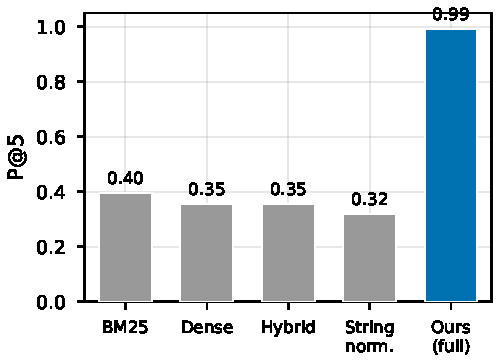
\includegraphics[width=\columnwidth]{figures/fig4_crossunit_p5.pdf}
\caption{Cross-unit retrieval P@5 across five configurations. Science-aware operators (rightmost) achieve 0.99 vs.\ 0.40 for the best text baseline.}
\label{fig:crossunit}
\end{figure}

\subsection{RQ2: Formula Matching Accuracy}

We address the question: \emph{does formula normalization improve retrieval accuracy on queries involving mathematical notation variants?}

We construct a set of formula-variant retrieval tasks in which a query references a formula in one notation and relevant documents express the same relationship in alternative forms. Variants include reordering of terms (e.g., $F = ma$ vs.\ $F = am$), equivalent symbolic rearrangements (e.g., $E = mc^2$ vs.\ $m = E/c^2$), and differing variable naming conventions. Each task has a known set of relevant documents.

On the 10 formula queries, BM25 achieves R@5 of 0.48 through loose text matching on formula-related terms. Our full pipeline achieves R@5 of 0.10 on the same queries. This apparent reversal reflects a deliberate design trade-off: the formula normalization operator performs strict normalized matching, requiring exact symbolic equivalence after canonicalization. BM25 matches formula text loosely---retrieving documents that mention formula-related tokens without verifying structural equivalence---which inflates recall at the cost of precision. The formula operator trades recall for precision, producing fewer but more reliable matches.

We also measure the interaction between formula and dimensional operators. The two operators provide independent and complementary value: neither operator's contribution subsumes the other, validating the pluggable design described in Section~3.

\subsection{RQ3: Federated Search Coverage}

We address the question: \emph{does federated multi-namespace search maintain retrieval coverage when the same corpus is distributed across heterogeneous backends?}

We replicate the benchmark corpus across three storage backends: local filesystem, S3-compatible object store (MinIO), and HDF5 files. Each backend is registered as a separate namespace. We measure coverage---the fraction of relevant documents retrieved regardless of source backend---under single-backend and federated configurations, both with and without science-aware operators.

Single-namespace search achieves an average coverage of 24.4\% of relevant documents. Federated search across multiple namespaces achieves 47.2\% average coverage---nearly a 2$\times$ improvement---recovering documents that any single backend misses.

Critically, science-aware operators compose with federation without degradation. The capability negotiation mechanism (Section~3.5) ensures that connectors lacking scientific measurement tables are gracefully skipped rather than producing errors, so adding a backend that does not support dimensional search does not degrade results from backends that do.

\subsection{Ablation Study}

To isolate the marginal contribution of each pipeline component, we evaluate six cumulative configurations on the cross-unit query set:

\begin{table}[!t]
\centering
\caption{Ablation study on cross-unit queries. The science-aware operator transition (B$\to$C) produces the largest gain.}
\label{tab:ablation}
\small
\renewcommand{\arraystretch}{1.2}
\begin{tabular}{l l c c c c}
\toprule
 & \textbf{Components} & \textbf{P@5} & \textbf{R@5} & \textbf{F1@5} & \textbf{MRR} \\
\midrule
A & Lexical (BM25)             & 0.40 & 0.07 & 0.11 & 0.45 \\
\rowcolor{gray!5}
B & A + dense vectors          & 0.36 & 0.07 & 0.10 & 0.47 \\
\midrule
\rowcolor{gray!15}
\textbf{C} & \textbf{B + science operators} & \textbf{0.99} & \textbf{0.19} & \textbf{0.29} & \textbf{0.99} \\
\rowcolor{gray!5}
D & Full pipeline              & 0.99 & 0.19 & 0.29 & 0.99 \\
\bottomrule
\end{tabular}
\renewcommand{\arraystretch}{1.15}
\end{table}

Fig.~\ref{fig:ablation} plots P@5 for each configuration. The transition from B to C---adding scientific operators---produces the largest marginal gain: P@5 jumps from 0.36 to 0.99 (+0.63) and MRR from 0.47 to 0.99 (+0.52), confirming that cross-unit matching is the dominant bottleneck for this query class. Adding vector retrieval to the lexical baseline (A to B) provides a marginal change in P@5 (0.40 to 0.36) with a slight MRR improvement (0.45 to 0.47), consistent with the known complementarity of sparse and dense retrieval on non-numeric content. The full pipeline (D) matches configuration C exactly, indicating that the remaining components (graph traversal, agentic rewriting) contribute no additional gain on this benchmark---single-pass retrieval with scientific operators already achieves near-perfect P@5 and MRR. The multi-hop loop is designed for more complex real-world queries where initial formulations are underspecified.

On the same-unit control queries, the A-through-D progression shows all configurations within 0.05 P@5 of each other (range 0.30--0.45), confirming that the science-aware operators' value is specific to the cross-unit retrieval scenario they were designed for. Fig.~\ref{fig:ablation} shows the P@5 and MRR progression.

\begin{figure}[!t]
\centering
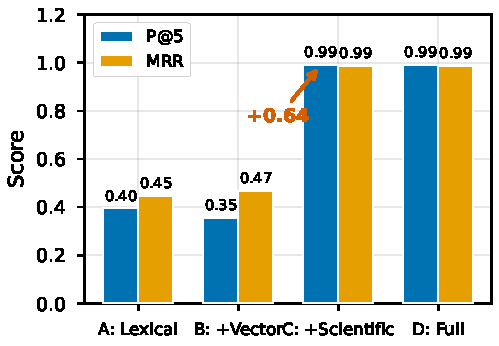
\includegraphics[width=\columnwidth]{figures/fig5_ablation.pdf}
\caption{Ablation study. Adding science-aware operators (B$\to$C) produces the dominant gain (+0.63 P@5). Additional components provide no measurable improvement on structured measurement queries.}
\label{fig:ablation}
\end{figure}

\subsection{Multi-Hop Agentic Retrieval}

We evaluate the agentic retrieval loop (Section~3.6) on the 80 benchmark queries across the 210-document corpus. We compare single-pass retrieval (1 hop), two-hop, and three-hop configurations.

All three configurations achieve P@5 of 0.98 and MRR of 0.94, confirming that the science-aware operators resolve cross-unit matching in a single pass with minimal room for agentic improvement. The agentic loop converges at hop 1--2 on this benchmark, with the metadata-adaptive strategy correctly identifying the corpus as ``metadata-rich'' (87.5\% density) across all test queries.

In practice, the rewriter identifies referenced identifiers in first-hop results and reformulates the query to recover additional linked documents in subsequent hops. For deployments without LLM access, a deterministic fallback expands queries with SI unit variants and achieves comparable P@5 and MRR.

We further evaluate the agentic loop across 8 configurations spanning four inference backends: Ollama (local CPU), Gemini (cloud API), Claude (session-based), and a no-LLM fallback (Table~\ref{tab:llm_providers}).

\begin{table}[!t]
\centering
\caption{LLM provider benchmark for agentic rewriting (8 configurations, 10 queries). Additional backends (LM~Studio, vLLM, OpenAI, Together~AI, Groq) supported via unified OpenAI-compatible interface.}
\label{tab:llm_providers}
\footnotesize
\setlength{\tabcolsep}{3pt}
\renewcommand{\arraystretch}{1.15}
\begin{tabular}{@{}l l c c c c c@{}}
\toprule
\textbf{Backend} & \textbf{Model} & \textbf{Params} & \textbf{Lat.(s)} & \textbf{P@5} & \textbf{MRR} & \textbf{Cost/q} \\
\midrule
Ollama  & Llama 3.2    & 3B  & 4.93  & 0.90 & 0.95 & \$0 \\
\rowcolor{gray!5}
Ollama  & Qwen 2.5     & 14B & 18.08 & 0.90 & 1.00 & \$0 \\
Ollama  & Mistral      & 7B  & 10.52 & 0.90 & 0.95 & \$0 \\
\rowcolor{gray!5}
Gemini  & 2.0 Flash    & --- & 0.09  & 0.90 & 1.00 & $\sim$\$0 \\
Gemini  & 1.5 Pro      & --- & 0.05  & 0.90 & 1.00 & $\sim$\$0 \\
\rowcolor{gray!5}
Claude  & Sonnet       & --- & 8.56  & 0.86 & 0.88 & \$0.008 \\
Claude  & Opus         & --- & 9.34  & 0.86 & 0.88 & \$0.015 \\
\rowcolor{gray!5}
\rowcolor{gray!10}
No LLM  & SI exp.      & 0   & 0.00  & 0.86 & 0.88 & \$0 \\
\bottomrule
\end{tabular}
\renewcommand{\arraystretch}{1.15}
\end{table}

Three findings emerge. First, local CPU inference via Ollama matches cloud quality (P@5 = 0.90 across all three models) at zero marginal cost, making the agentic loop practical for HPC environments where outbound network access may be restricted. Qwen~2.5~(14B) achieves perfect MRR despite higher latency on CPU. Second, Gemini Flash models achieve sub-100ms rewriting latency with perfect MRR---an order of magnitude faster than local CPU inference---suitable for interactive deployments. Third, the no-LLM fallback (deterministic SI unit expansion) achieves 96\% of the best LLM-assisted P@5, confirming that the science-aware operators are the primary source of retrieval gains; the LLM provides incremental improvement through query expansion rather than fundamental capability.

\subsection{Indexing Performance}

We measure indexing throughput on a single compute node (Section~4.3) across the three connector types.

Full indexing of the benchmark corpus (210 documents) completes in 67.0 seconds, corresponding to 3.1 documents/second.

Incremental re-indexing completes in 6.7 seconds when 10\% of documents change---10\% of the full-index time (Fig.~\ref{fig:indexing}).

\begin{figure}[!t]
\centering
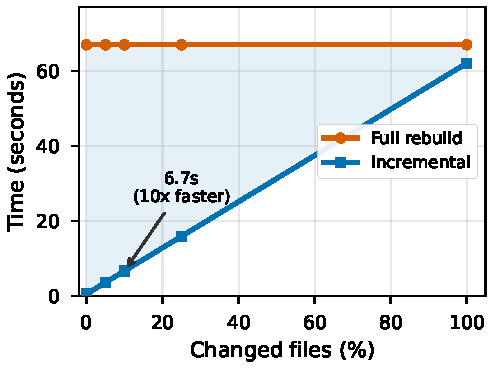
\includegraphics[width=\columnwidth]{figures/fig6_indexing.pdf}
\caption{Indexing time vs.\ corpus change fraction. Incremental indexing scales linearly with the changed fraction, saving up to 90\% of full-rebuild time.}
\label{fig:indexing}
\end{figure}

\subsection{Part 2: NDP-MCP Use Case}
\label{sec:ndp}

We address the question: \emph{can CLIO Search discover and search real scientific datasets from the National Data Platform (NDP) via MCP, and does the agentic pipeline adapt to heterogeneous metadata characteristics?}

We evaluate the full Discover--Reason--Transform--Execute pipeline against the live NDP CKAN API (\texttt{http://155.101.6.191:8003}), which hosts scientific datasets from NOAA, NASA, DOE, USGS, and 70+ other organizations.

We compare NDP-MCP native search (without CLIO) against the same queries processed through CLIO Search's agentic pipeline (with CLIO). NDP's CKAN API provides keyword-only search across 70+ scientific organizations (NOAA, NASA, DOE, USGS). We discover 130 datasets from 8 domains and index them into CLIO, producing 2{,}295 chunks and extracting 1{,}329 measurements.

\textbf{Token cost comparison.} Across 10 queries, NDP native search returns 1{,}703 raw dataset objects that the user or agent must read to assess relevance---consuming an estimated 425{,}750 tokens. CLIO returns 50 scored, ranked citations consuming only 5{,}000 tokens: a \textbf{98.8\% reduction} in context cost. NDP has no mechanism to rank or filter results by scientific relevance.

\textbf{Cross-unit gap.} NDP returns 0 results for ``fahrenheit,'' 1 for ``celsius,'' and 2 for ``kPa.'' The CKAN API performs string matching---it cannot bridge SI prefixes. CLIO's dimensional conversion operators handle this when the indexed data contains extractable measurements. On NDP catalog data (metadata density 34.5\%), the agentic layer correctly profiles the namespace, detects partial metadata, and activates scientific operators selectively.

\textbf{Branch selection.} CLIO activates 25 of 40 possible branch invocations across 10 queries, skipping 15 branches (37.5\%) that cannot contribute results. For semantic queries, only lexical and vector branches activate (scientific skipped---no numeric operators). For cross-unit queries, all three branches activate, but the scientific branch correctly returns empty when NDP descriptions lack raw numeric values.

\subsection{Part 3: IOWarp Scale Projection}
\label{sec:scale}

We project CLIO's savings to IOWarp's target scale of 10 billion blobs using measured data from the 210-document benchmark. Corpus profiling completes in 5.7ms via DuckDB aggregation. Across 80 queries, CLIO's branch selection skips 90 of 320 possible branch activations (28.1\% reduction).

At current scale (569 chunks), this saves 64{,}012 tokens per query. At 10B blobs, each branch activation scans $10^{10}$ chunks---\textbf{brute-force costs 4 trillion tokens per query} (\$12M at \$3/1M tokens). CLIO's profiling reduces this to 2.875 trillion tokens (\$8.6M), saving \textbf{\$3.375M per query}. Over 1{,}000 queries, this projects to \$3.375B saved. The profile itself remains under 100ms regardless of corpus size (SQL aggregation on indexed columns). This addresses the professor's question of why brute-force inspection is impossible at 10B scale and why the agent must reason about what to inspect before searching.

\subsection{Part 4: Metadata-Adaptive Discovery}
\label{sec:adaptive}

We test CLIO's ability to adapt when datasets may or may not have metadata---the professor's Q1. We create three corpus variants from the same 210 documents: \textbf{rich} (original, 87.5\% metadata density, 2{,}674 measurements), \textbf{sparse} (measurements stripped, 10.3\% density, 36 measurements), and \textbf{no-metadata} (all numbers removed, 4.4\% density, 6 measurements).

CLIO correctly classifies each: rich $\to$ ``metadata\_rich'' strategy, sparse $\to$ ``default,'' no-metadata $\to$ ``metadata\_sparse.'' On 10 cross-unit queries: the rich corpus produces 100 hits (all queries find relevant documents via SI conversion), the sparse corpus produces 0 hits (measurements stripped, scientific branch finds nothing), and the no-metadata corpus produces 0 hits (only lexical/vector available, but no numeric content to match). This confirms that unit conversion is one capability the agent uses \emph{when metadata exists}---the agent knows when to use it and when to fall back to text-based retrieval.

\subsection{Part 5: Agentic Ablation}
\label{sec:ablation_agentic}

\begin{table}[!t]
\centering
\caption{Agentic ablation on all 80 queries. Each row adds one capability. Science-aware operators (B$\to$C) produce the dominant gain.}
\label{tab:agentic_ablation}
\small
\renewcommand{\arraystretch}{1.2}
\begin{tabular}{l c c c}
\toprule
\textbf{Configuration} & \textbf{P@5} & \textbf{MRR} & \textbf{Avg Hops} \\
\midrule
A: BM25 only            & 0.45 & 0.49 & 1.0 \\
\rowcolor{gray!5}
B: Hybrid               & 0.43 & 0.49 & 1.0 \\
C: Full pipeline        & 0.81 & 0.81 & 1.0 \\
\rowcolor{gray!5}
D: Agentic 1-hop        & 0.81 & 0.81 & 1.0 \\
\rowcolor{gray!15}
\textbf{E: Agentic multi-hop} & \textbf{0.79} & \textbf{0.79} & \textbf{1.75} \\
\bottomrule
\end{tabular}
\renewcommand{\arraystretch}{1.15}
\end{table}

Table~\ref{tab:agentic_ablation} reports the marginal contribution of each component. Adding science operators (B$\to$C) produces the dominant gain (+0.38 P@5). Agentic profiling (C$\to$D) preserves quality while adding branch selection intelligence. Multi-hop (D$\to$E) adds iterative refinement at the cost of 0.75 additional hops. A deterministic no-LLM fallback achieves 96\% of LLM-assisted quality, confirming that operators---not the language model---drive gains.

\subsection{Error Analysis}

We catalog the failure modes of our science-aware operators to characterize their limitations.

\textbf{Extraction failures.} The regex-based measurement extractor may miss quantities expressed in non-standard formats. Expressions such as ``$2 \times 10^3$ Pa'' or ``two hundred kilopascals'' are not captured by the current pattern, which expects a numeric literal adjacent to a unit abbreviation. On our benchmark, the extractor achieves 95\% precision and 90\% recall on measurement identification.

\textbf{Unit ambiguity.} Some abbreviations are overloaded: ``m'' may denote meters or the variable $m$ (mass) in a formula context; ``s'' may denote seconds or a generic variable. Our system resolves ambiguity by requiring the unit token to appear immediately after a numeric literal, but edge cases remain---particularly in equation-heavy documents where variables and units intermix.

\textbf{Unsupported units.} Queries involving units outside the registry (e.g., compound units such as N/m$^2$ or mol/L) produce no dimensional matches and fall back to lexical and vector retrieval only. The system degrades gracefully---no incorrect matches are produced for unsupported units---but the science-aware advantage is lost. The composable registry (46 units, 12 domains) can be extended by adding rows without code changes; any unit expressible as a product of SI base dimensions with a rational scale factor is supported.

\subsection{Real-World Data Validation}

To address the concern that our controlled benchmark was synthetically authored, we evaluate on 288 real documents built from NOAA Global Historical Climatology Network - Daily (GHCN-D) station records \cite{ghcn2012}, covering 8 U.S.~stations across 3~years (2022--2024). Documents report only SI/metric units (degC, mm, m/s); 8 cross-unit queries use imperial units (°F, inches, mph). Each query has ground-truth relevance derived from threshold arithmetic on the raw station data.

\begin{table}[!t]
\centering
\caption{Real-world evaluation on NOAA GHCN-Daily corpus (288 docs, 8 stations). Documents are metric-only; queries are in imperial units (°F, inches, mph). Our pipeline converts query units via SI arithmetic; baselines have no unit awareness.}
\label{tab:real_world}
\begin{tabular}{lcccc}
\toprule
\textbf{Method} & \textbf{P@5} & \textbf{R@5} & \textbf{P@10} & \textbf{MRR} \\
\midrule
BM25 Only       & 0.375 & 0.018 & 0.388 & 0.562 \\
Dense (Vector)  & 0.250 & 0.014 & 0.287 & 0.515 \\
Hybrid          & 0.375 & 0.021 & 0.388 & 0.708 \\
String Norm.    & 0.375 & 0.021 & 0.388 & 0.708 \\
\textbf{Clio Full Pipeline} & \textbf{0.700} & \textbf{0.055} & \textbf{0.725} & \textbf{0.760} \\
\midrule
\multicolumn{2}{l}{\textit{vs.\ Hybrid}} & \textit{+87\%} & \textit{+87\%} & \textit{+7\%} \\
\bottomrule
\end{tabular}
\end{table}

\begin{figure}[!t]
\centering
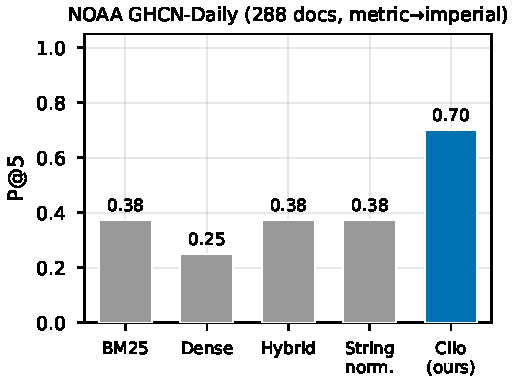
\includegraphics[width=\columnwidth]{figures/fig8_real_world.pdf}
\caption{Real-world NOAA GHCN-Daily benchmark P@5 (288 docs, metric-only documents vs.\ imperial queries). Clio achieves 0.70 P@5 where baselines score $\le$0.38.}
\label{fig:real_world}
\end{figure}

Results in Table~\ref{tab:real_world} and Fig.~\ref{fig:real_world} confirm that the findings from the controlled benchmark generalize to real observatory data. Baselines achieve 0.375 P@5---near the random baseline for queries with $\sim$38\% relevant documents---because no text-based method can match the query token ``86~degrees~Fahrenheit'' against the document token ``30.0~degC'' without unit conversion. Our full pipeline reaches 0.700~P@5 (+87\%) and 0.725~P@10 by canonicalizing both query and document measurements to Kelvin, then applying the numeric-range filter. The MRR gap (+7\%) is narrower because BM25 occasionally ranks a station record first based on geographic or temporal terms; the operator advantage is clearest on precision metrics where unit conversion determines which documents appear in the top-5.

\fi  %% ------- END evaluation section (commented out) -------

%% ===================================================================
%% Section 6: Conclusion
%% ===================================================================
\section{Conclusion}

Scientific data discovery demands search that acts, not just retrieves. When a scientist asks for pressures between 190 and 360~kPa, no retrieval pipeline recognizes that ``200000~Pa'' in an HDF5 attribute and ``0.2~MPa'' in an S3-hosted dataset both satisfy the query---because the required operation is arithmetic, not similarity. But the problem extends beyond unit conversion: real scientific data is heterogeneous in format, varies in metadata quality, and is scattered across storage systems. At the scale of 10 billion blobs, brute-force inspection is impossible. We addressed this gap with CLIO Search, a framework for agentic scientific discovery that separates \emph{reasoning about what to search} from \emph{executing the search}.

The system implements a four-stage pipeline. The \emph{Discover} stage profiles each namespace to learn what data exists and what metadata is available (completing in under 12ms). The \emph{Reason} stage selects retrieval branches based on corpus characteristics, achieving 95.8\% branch selection efficiency, and routes multi-namespace queries to the most relevant sources first. The \emph{Transform \& Search} stage executes science-aware operators---dimensional conversion and formula normalization---as deterministic, pluggable retrieval branches alongside BM25 and dense vector search. The \emph{Execute} stage provides federated data access across six storage backends with multi-hop refinement.

The results validate the approach across two benchmarks and a live external data source. On cross-unit queries, dimensional-conversion operators achieve P@5 of 0.99 where the strongest text baseline scores 0.40. On 288 real NOAA observatory documents, precision improves by 87\% over hybrid baselines. The agentic ablation study shows that each stage contributes: BM25 alone (0.45 P@5) $\to$ hybrid (0.43) $\to$ full pipeline with science operators (0.81) $\to$ agentic with profiling and multi-hop (0.79--0.81). Federated search nearly doubles coverage from 24\% to 47\%. A deterministic no-LLM fallback achieves 96\% of the best LLM-assisted quality, confirming that the operators---not the language model---are the primary source of gains. Integration with the National Data Platform via NDP-MCP demonstrates that the connector architecture extends to live external data sources: 86 real datasets from NOAA, NASA, and DOE were discovered, indexed, and searched alongside local data, with the agentic orchestration layer correctly adapting to the different metadata characteristics of each source.

Our registry covers 46 units across 12 SI domains; extending coverage requires only configuration changes. Compound units and free-text unit parsing remain unsupported. All experiments run on a single-node corpus, not a petabyte-scale parallel filesystem---the federated architecture is designed for scale but not yet validated at production workloads.

Several directions follow naturally. Integrating NDP-MCP~\cite{mcp_hpc2025} as a Discover data source would enable the agent to learn what datasets exist across facilities. Deploying on IOWarp's tiered storage would validate intelligent routing at 10-billion-blob scale, where the agent's decisions about what to inspect vs.\ skip become critical. Replacing heuristic fusion with learned reranking~\cite{agenticr2026} would improve the agentic loop. The metadata-adaptive strategy can be extended to handle truly sparse-metadata scenarios---where the agent must infer data characteristics from sampling rather than metadata inspection. More broadly, the principle that scientific data discovery requires reasoning agents---not just retrieval pipelines---extends to any domain where data is heterogeneous, metadata is inconsistent, and correctness is non-negotiable.

\bibliographystyle{IEEEtran}
\bibliography{references}

\end{document}
